% Options for packages loaded elsewhere
\PassOptionsToPackage{unicode}{hyperref}
\PassOptionsToPackage{hyphens}{url}
\PassOptionsToPackage{dvipsnames,svgnames,x11names}{xcolor}
%
\documentclass[
  letterpaper,
  DIV=11,
  numbers=noendperiod]{scrartcl}

\usepackage{amsmath,amssymb}
\usepackage{iftex}
\ifPDFTeX
  \usepackage[T1]{fontenc}
  \usepackage[utf8]{inputenc}
  \usepackage{textcomp} % provide euro and other symbols
\else % if luatex or xetex
  \usepackage{unicode-math}
  \defaultfontfeatures{Scale=MatchLowercase}
  \defaultfontfeatures[\rmfamily]{Ligatures=TeX,Scale=1}
\fi
\usepackage{lmodern}
\ifPDFTeX\else  
    % xetex/luatex font selection
\fi
% Use upquote if available, for straight quotes in verbatim environments
\IfFileExists{upquote.sty}{\usepackage{upquote}}{}
\IfFileExists{microtype.sty}{% use microtype if available
  \usepackage[]{microtype}
  \UseMicrotypeSet[protrusion]{basicmath} % disable protrusion for tt fonts
}{}
\makeatletter
\@ifundefined{KOMAClassName}{% if non-KOMA class
  \IfFileExists{parskip.sty}{%
    \usepackage{parskip}
  }{% else
    \setlength{\parindent}{0pt}
    \setlength{\parskip}{6pt plus 2pt minus 1pt}}
}{% if KOMA class
  \KOMAoptions{parskip=half}}
\makeatother
\usepackage{xcolor}
\setlength{\emergencystretch}{3em} % prevent overfull lines
\setcounter{secnumdepth}{-\maxdimen} % remove section numbering
% Make \paragraph and \subparagraph free-standing
\ifx\paragraph\undefined\else
  \let\oldparagraph\paragraph
  \renewcommand{\paragraph}[1]{\oldparagraph{#1}\mbox{}}
\fi
\ifx\subparagraph\undefined\else
  \let\oldsubparagraph\subparagraph
  \renewcommand{\subparagraph}[1]{\oldsubparagraph{#1}\mbox{}}
\fi

\usepackage{color}
\usepackage{fancyvrb}
\newcommand{\VerbBar}{|}
\newcommand{\VERB}{\Verb[commandchars=\\\{\}]}
\DefineVerbatimEnvironment{Highlighting}{Verbatim}{commandchars=\\\{\}}
% Add ',fontsize=\small' for more characters per line
\usepackage{framed}
\definecolor{shadecolor}{RGB}{241,243,245}
\newenvironment{Shaded}{\begin{snugshade}}{\end{snugshade}}
\newcommand{\AlertTok}[1]{\textcolor[rgb]{0.68,0.00,0.00}{#1}}
\newcommand{\AnnotationTok}[1]{\textcolor[rgb]{0.37,0.37,0.37}{#1}}
\newcommand{\AttributeTok}[1]{\textcolor[rgb]{0.40,0.45,0.13}{#1}}
\newcommand{\BaseNTok}[1]{\textcolor[rgb]{0.68,0.00,0.00}{#1}}
\newcommand{\BuiltInTok}[1]{\textcolor[rgb]{0.00,0.23,0.31}{#1}}
\newcommand{\CharTok}[1]{\textcolor[rgb]{0.13,0.47,0.30}{#1}}
\newcommand{\CommentTok}[1]{\textcolor[rgb]{0.37,0.37,0.37}{#1}}
\newcommand{\CommentVarTok}[1]{\textcolor[rgb]{0.37,0.37,0.37}{\textit{#1}}}
\newcommand{\ConstantTok}[1]{\textcolor[rgb]{0.56,0.35,0.01}{#1}}
\newcommand{\ControlFlowTok}[1]{\textcolor[rgb]{0.00,0.23,0.31}{#1}}
\newcommand{\DataTypeTok}[1]{\textcolor[rgb]{0.68,0.00,0.00}{#1}}
\newcommand{\DecValTok}[1]{\textcolor[rgb]{0.68,0.00,0.00}{#1}}
\newcommand{\DocumentationTok}[1]{\textcolor[rgb]{0.37,0.37,0.37}{\textit{#1}}}
\newcommand{\ErrorTok}[1]{\textcolor[rgb]{0.68,0.00,0.00}{#1}}
\newcommand{\ExtensionTok}[1]{\textcolor[rgb]{0.00,0.23,0.31}{#1}}
\newcommand{\FloatTok}[1]{\textcolor[rgb]{0.68,0.00,0.00}{#1}}
\newcommand{\FunctionTok}[1]{\textcolor[rgb]{0.28,0.35,0.67}{#1}}
\newcommand{\ImportTok}[1]{\textcolor[rgb]{0.00,0.46,0.62}{#1}}
\newcommand{\InformationTok}[1]{\textcolor[rgb]{0.37,0.37,0.37}{#1}}
\newcommand{\KeywordTok}[1]{\textcolor[rgb]{0.00,0.23,0.31}{#1}}
\newcommand{\NormalTok}[1]{\textcolor[rgb]{0.00,0.23,0.31}{#1}}
\newcommand{\OperatorTok}[1]{\textcolor[rgb]{0.37,0.37,0.37}{#1}}
\newcommand{\OtherTok}[1]{\textcolor[rgb]{0.00,0.23,0.31}{#1}}
\newcommand{\PreprocessorTok}[1]{\textcolor[rgb]{0.68,0.00,0.00}{#1}}
\newcommand{\RegionMarkerTok}[1]{\textcolor[rgb]{0.00,0.23,0.31}{#1}}
\newcommand{\SpecialCharTok}[1]{\textcolor[rgb]{0.37,0.37,0.37}{#1}}
\newcommand{\SpecialStringTok}[1]{\textcolor[rgb]{0.13,0.47,0.30}{#1}}
\newcommand{\StringTok}[1]{\textcolor[rgb]{0.13,0.47,0.30}{#1}}
\newcommand{\VariableTok}[1]{\textcolor[rgb]{0.07,0.07,0.07}{#1}}
\newcommand{\VerbatimStringTok}[1]{\textcolor[rgb]{0.13,0.47,0.30}{#1}}
\newcommand{\WarningTok}[1]{\textcolor[rgb]{0.37,0.37,0.37}{\textit{#1}}}

\providecommand{\tightlist}{%
  \setlength{\itemsep}{0pt}\setlength{\parskip}{0pt}}\usepackage{longtable,booktabs,array}
\usepackage{calc} % for calculating minipage widths
% Correct order of tables after \paragraph or \subparagraph
\usepackage{etoolbox}
\makeatletter
\patchcmd\longtable{\par}{\if@noskipsec\mbox{}\fi\par}{}{}
\makeatother
% Allow footnotes in longtable head/foot
\IfFileExists{footnotehyper.sty}{\usepackage{footnotehyper}}{\usepackage{footnote}}
\makesavenoteenv{longtable}
\usepackage{graphicx}
\makeatletter
\def\maxwidth{\ifdim\Gin@nat@width>\linewidth\linewidth\else\Gin@nat@width\fi}
\def\maxheight{\ifdim\Gin@nat@height>\textheight\textheight\else\Gin@nat@height\fi}
\makeatother
% Scale images if necessary, so that they will not overflow the page
% margins by default, and it is still possible to overwrite the defaults
% using explicit options in \includegraphics[width, height, ...]{}
\setkeys{Gin}{width=\maxwidth,height=\maxheight,keepaspectratio}
% Set default figure placement to htbp
\makeatletter
\def\fps@figure{htbp}
\makeatother
% definitions for citeproc citations
\NewDocumentCommand\citeproctext{}{}
\NewDocumentCommand\citeproc{mm}{%
  \begingroup\def\citeproctext{#2}\cite{#1}\endgroup}
\makeatletter
 % allow citations to break across lines
 \let\@cite@ofmt\@firstofone
 % avoid brackets around text for \cite:
 \def\@biblabel#1{}
 \def\@cite#1#2{{#1\if@tempswa , #2\fi}}
\makeatother
\newlength{\cslhangindent}
\setlength{\cslhangindent}{1.5em}
\newlength{\csllabelwidth}
\setlength{\csllabelwidth}{3em}
\newenvironment{CSLReferences}[2] % #1 hanging-indent, #2 entry-spacing
 {\begin{list}{}{%
  \setlength{\itemindent}{0pt}
  \setlength{\leftmargin}{0pt}
  \setlength{\parsep}{0pt}
  % turn on hanging indent if param 1 is 1
  \ifodd #1
   \setlength{\leftmargin}{\cslhangindent}
   \setlength{\itemindent}{-1\cslhangindent}
  \fi
  % set entry spacing
  \setlength{\itemsep}{#2\baselineskip}}}
 {\end{list}}
\usepackage{calc}
\newcommand{\CSLBlock}[1]{\hfill\break\parbox[t]{\linewidth}{\strut\ignorespaces#1\strut}}
\newcommand{\CSLLeftMargin}[1]{\parbox[t]{\csllabelwidth}{\strut#1\strut}}
\newcommand{\CSLRightInline}[1]{\parbox[t]{\linewidth - \csllabelwidth}{\strut#1\strut}}
\newcommand{\CSLIndent}[1]{\hspace{\cslhangindent}#1}

\usepackage{fontspec}
\usepackage{multirow}
\usepackage{multicol}
\usepackage{colortbl}
\usepackage{hhline}
\newlength\Oldarrayrulewidth
\newlength\Oldtabcolsep
\usepackage{longtable}
\usepackage{array}
\usepackage{hyperref}
\usepackage{float}
\usepackage{wrapfig}
\KOMAoption{captions}{tableheading}
\makeatletter
\@ifpackageloaded{tcolorbox}{}{\usepackage[skins,breakable]{tcolorbox}}
\@ifpackageloaded{fontawesome5}{}{\usepackage{fontawesome5}}
\definecolor{quarto-callout-color}{HTML}{909090}
\definecolor{quarto-callout-note-color}{HTML}{0758E5}
\definecolor{quarto-callout-important-color}{HTML}{CC1914}
\definecolor{quarto-callout-warning-color}{HTML}{EB9113}
\definecolor{quarto-callout-tip-color}{HTML}{00A047}
\definecolor{quarto-callout-caution-color}{HTML}{FC5300}
\definecolor{quarto-callout-color-frame}{HTML}{acacac}
\definecolor{quarto-callout-note-color-frame}{HTML}{4582ec}
\definecolor{quarto-callout-important-color-frame}{HTML}{d9534f}
\definecolor{quarto-callout-warning-color-frame}{HTML}{f0ad4e}
\definecolor{quarto-callout-tip-color-frame}{HTML}{02b875}
\definecolor{quarto-callout-caution-color-frame}{HTML}{fd7e14}
\makeatother
\makeatletter
\@ifpackageloaded{caption}{}{\usepackage{caption}}
\AtBeginDocument{%
\ifdefined\contentsname
  \renewcommand*\contentsname{Table of contents}
\else
  \newcommand\contentsname{Table of contents}
\fi
\ifdefined\listfigurename
  \renewcommand*\listfigurename{List of Figures}
\else
  \newcommand\listfigurename{List of Figures}
\fi
\ifdefined\listtablename
  \renewcommand*\listtablename{List of Tables}
\else
  \newcommand\listtablename{List of Tables}
\fi
\ifdefined\figurename
  \renewcommand*\figurename{Figure}
\else
  \newcommand\figurename{Figure}
\fi
\ifdefined\tablename
  \renewcommand*\tablename{Table}
\else
  \newcommand\tablename{Table}
\fi
}
\@ifpackageloaded{float}{}{\usepackage{float}}
\floatstyle{ruled}
\@ifundefined{c@chapter}{\newfloat{codelisting}{h}{lop}}{\newfloat{codelisting}{h}{lop}[chapter]}
\floatname{codelisting}{Listing}
\newcommand*\listoflistings{\listof{codelisting}{List of Listings}}
\makeatother
\makeatletter
\makeatother
\makeatletter
\@ifpackageloaded{caption}{}{\usepackage{caption}}
\@ifpackageloaded{subcaption}{}{\usepackage{subcaption}}
\makeatother
\ifLuaTeX
  \usepackage{selnolig}  % disable illegal ligatures
\fi
\usepackage{bookmark}

\IfFileExists{xurl.sty}{\usepackage{xurl}}{} % add URL line breaks if available
\urlstyle{same} % disable monospaced font for URLs
\hypersetup{
  pdftitle={Regresión lineal simple (RLS)},
  colorlinks=true,
  linkcolor={blue},
  filecolor={Maroon},
  citecolor={Blue},
  urlcolor={Blue},
  pdfcreator={LaTeX via pandoc}}

\title{\textbf{Regresión lineal simple (RLS)}}
\author{}
\date{}

\begin{document}
\maketitle

{Este material es parte de la \textbf{Unidad 3 del Curso de
Epidemiología - Nivel Avanzado del Instituto Nacional de Epidemiología
``Dr.~Juan H. Jara'' - ANLIS}}

{\href{https://datos-ine.github.io/EpiAvanzada/unidad_3/rls/}{Regresión
lineal simple} by \hyperref[0]{Andrea Silva, Christian Ballejo y Tamara
Ricardo} is licensed under \hyperref[0]{CC BY-NC 4.0} }

\subsection{Covarianza y correlación}\label{covarianza-y-correlaciuxf3n}

Nuestra pregunta ahora es: ¿cómo podemos estudiar la relación de dos
variables cuantitativas que varían simultáneamente (co-varían), una en
función de la otra?

AI analizar los datos en las disciplinas que conforman las ciencias de
la salud, con frecuencia es conveniente obtener algún conocimiento
acerca de la relación entre dos variables. Por ejemplo, es posible que
se tenga interés en analizar la relación entre presión sanguínea y edad,
estatura y peso, la concentración de un medicamento inyectable y la
frecuencia cardíaca, etc (observar que se trata de variables
cuantitativas)

La \textbf{covarianza} \(S_{XY}\), es una medida que nos hablará de la
variabilidad conjunta de dos variables numéricas (cuantitativas). Se
define como:

\[S_{XY} = \frac{1}{n} \sum_{i=1}^{n} (x_i - \bar{x})(y_i - \bar{y})  \]

\textbf{¿Cómo se interpreta geométricamente la covarianza?}

Consideremos la nube de puntos formadas por las \(n\) parejas de datos
(\(x_i\), \(y_i\)). El centro de gravedad de esta nube de puntos es
(\(\bar{x}\) , \(\bar{y}\)). Trasladamos los ejes XY al nuevo centro de
coordenadas. Los puntos que se encuentran en el primer y tercer
cuadrante contribuyen positivamente al valor de \(S_{XY}\) , y los que
se encuentran en el segundo y el cuarto lo hacen negativamente.

\begin{center}
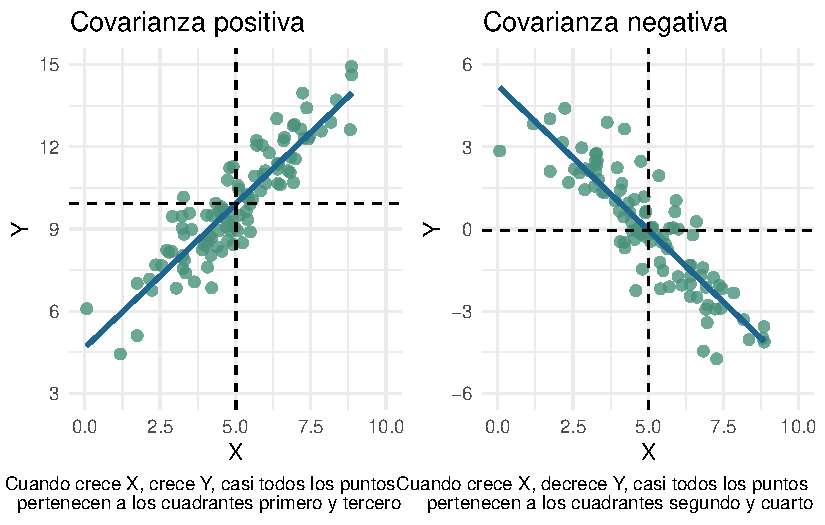
\includegraphics{index_files/figure-pdf/unnamed-chunk-2-1.pdf}
\end{center}

\begin{tcolorbox}[enhanced jigsaw, toptitle=1mm, colbacktitle=quarto-callout-important-color!10!white, opacitybacktitle=0.6, leftrule=.75mm, rightrule=.15mm, title=\textcolor{quarto-callout-important-color}{\faExclamation}\hspace{0.5em}{Importante}, colframe=quarto-callout-important-color-frame, breakable, coltitle=black, bottomrule=.15mm, opacityback=0, left=2mm, titlerule=0mm, bottomtitle=1mm, toprule=.15mm, colback=white, arc=.35mm]

\begin{itemize}
\item
  Si la mayoría de puntos se ubican en el tercer y primer cuadrante:
  \(S_{XY}\) \textgreater0
\item
  Si la mayoría de puntos se ubican en el segundo y cuarto cuadrante:
  \(S_{XY}\) \textless{} 0
\item
  Cuando los puntos se reparte de modo más o menos homogéneo entre los
  cuadrantes primero y tercero, y segundo y cuarto, se tiene que
  \(S_{XY}\) \textasciitilde{} 0.
\end{itemize}

\end{tcolorbox}

La covarianza es una medida de la variabilidad común de dos variables
(crecimiento de ambas al mismo tiempo o crecimiento de una y
decrecimiento de la otra), pero está afectada por las unidades en las
que cada variable se mide. Así pues, es necesario definir una medida de
la relación entre dos variables, y que no esté afectada por los cambios
de unidad de medida. Una forma de conseguir este objetivo es dividir la
covarianza por el producto de las desviaciones típicas de cada variable,
ya que así se obtiene un coeficiente adimensional, \(r\), que se
denomina coeficiente de \textbf{correlación lineal de Pearson}.

\[r = \frac{S_{XY}}{S_xS_y} \] Cuando hacemos un análisis bivariado de
nuestros datos, queremos determinar si parece haber una relación entre
las dos variables. Con frecuencia encontraremos una relación entre dos
variables al construir una gráfica: \textbf{diagrama de dispersión}.

Cuando examinamos un diagrama de dispersión, es necesario estudiar el
patrón general de los puntos graficados. Si existe un patrón, debemos
señalar su dirección. Es decir, mientras una variable se incrementa, ¿la
otra parece aumentar o disminuir? Tenemos que observar si hay datos
distantes, que son puntos que se ubican muy lejos de todos los demás.

La correlación trata de establecer la relación o dependencia que existe
entre las dos variables que intervienen en una distribución
bidimensional. Es decir, determinar si los cambios en una de las
variables influyen en los cambios de la otra. En caso de que suceda,
diremos que las variables están correlacionadas o que hay correlación
entre ellas.

La correlación, como cuantificación del grado de relación que hay entre
dos variables, es un valor entre -1 y +1, pasando, por el cero. Hay, por
lo tanto, correlaciones positivas y negativas. El signo es, pues, el
primer elemento básico a tener en cuenta.

Correlación positiva significa que las variables tienen una relación
directa: En este caso, valores pequeños de una variable van asociados a
valores también pequeños de la otra; y, paralelamente, valores grandes
de una van asociados a valores grandes de la otra.

La correlación negativa la tienen, por el contrario, variables con una
relación inversa. En este caso, valores pequeños de una variable van
asociados, ahora, a valores grandes de la otra; y, equivalentemente,
valores grandes de una van asociados a valores pequeños de la otra.

Lo segundo a tener en cuenta en la correlación es la magnitud. Y esto lo
marca el valor absoluto de la correlación. En la magnitud se valora la
correlación sin el signo, valorando la magnitud del número puro. Esto
significa que cuanto más cerca estemos de los extremos del intervalo de
valores posibles: -1 y +1, más correlación tenemos.

¿A partir de qué valores de \(r\) se considera que hay \emph{``buena
correlación''}? La respuesta no es simple. Hay que tener en cuenta la
presencia de observaciones anómalas y si la varianza se mantiene
homogénea. En reglas generales se acepta que a partir de 0,7 hay una
buena relación lineal y que a partir de 0,4 podría existir cierta
relación

\begin{tcolorbox}[enhanced jigsaw, toptitle=1mm, colbacktitle=quarto-callout-important-color!10!white, opacitybacktitle=0.6, leftrule=.75mm, rightrule=.15mm, title=\textcolor{quarto-callout-important-color}{\faExclamation}\hspace{0.5em}{En resumen}, colframe=quarto-callout-important-color-frame, breakable, coltitle=black, bottomrule=.15mm, opacityback=0, left=2mm, titlerule=0mm, bottomtitle=1mm, toprule=.15mm, colback=white, arc=.35mm]

\begin{itemize}
\item
  El \(r\) de Pearson es adimensional (su valor no depende de la unidad
  de medida de X e Y)
\item
  Sólo toma valores entre (-1 y +1)
\item
  Si \(r\) = 0 no existe asociación lineal entre \(x\) e \(y\) (pero
  cuidado: puede existir una asociación no-lineal). Cuando las variables
  son incorrelacionadas (hay independencia entre ellas), entonces \(r\)
  = 0.
\item
  Cuanto más cerca esté \(r\) de 1 o -1 mejor correlación
\end{itemize}

\end{tcolorbox}

La primera manera de explorar la relación entre 2 variables, es mediante
un gráfico o diagrama de dispersión que nos permite observar cómo se
comportan ambas variables. Luego se puede calcular el coeficiente de
correlación que nos dice si la relación es lineal y cuál es la fuerza de
esta correlación.

\begin{center}
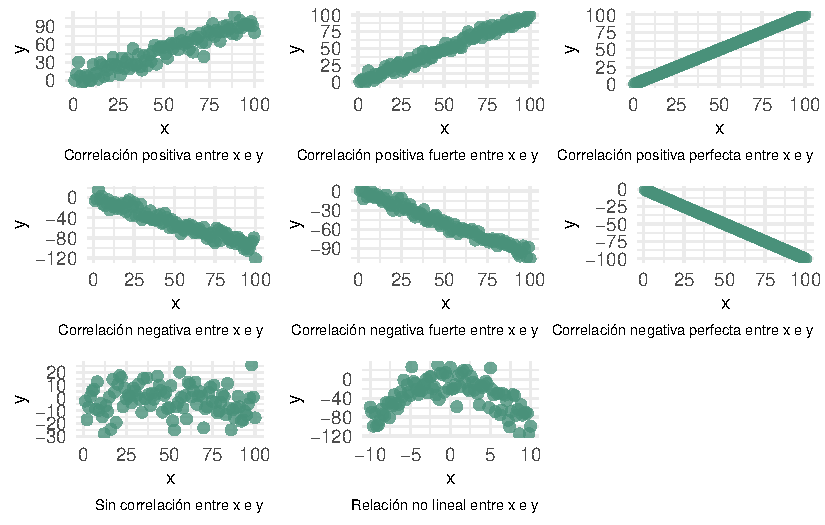
\includegraphics{index_files/figure-pdf/unnamed-chunk-3-1.pdf}
\end{center}

La correlación más usada para variables cuantitativas es la
\textbf{correlación de Pearson}. Es especialmente apropiada cuando la
distribución de las variables es la normal.

Si no se cumple la normalidad o si las variables son ordinales es más
apropiado usar la \textbf{correlación de Spearman} o la
\textbf{correlación de Kendall}.

Para explicar la forma de esta correlación e incluso predecir los
valores que puede alcanzar una variable (dependiente) en función de la
otra (independiente) podemos utilizar la \textbf{regresión lineal}.
Cuando el análisis lo realizamos con dos variables (una dependiente y
otra independiente) utilizamos la \textbf{regresión lineal simple}.
Cuando el problema es más complejo y queremos incorporar al análisis más
de una variable independiente utilizamos la \textbf{regresión lineal
múltiple}, que veremos más adelante.

Veamos un ejemplo:

A partir de los datos de peso (medido en gramos) y edad (medida en
semanas luego del nacimiento) de un set de datos ficticio con
información de 100 niñas menores de 6 meses se realizó un diagrama de
dispersión (\emph{``scatter plot''}).

\begin{figure}[H]

{\centering 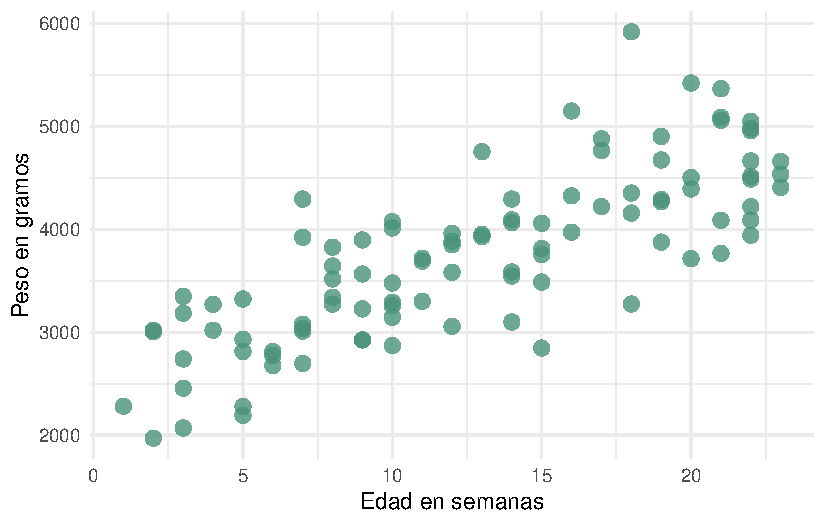
\includegraphics{index_files/figure-pdf/unnamed-chunk-4-1.pdf}

}

\caption{Gráfico 1. Edad y peso en 100 lactantes de sexo femenino.}

\end{figure}%

Como puede observarse existe una fuerte relación lineal positiva, donde
a medida que aumenta la edad aumenta el peso, si bien se observan
algunos casos que lo hacen con cierta variación.

En la segunda figura trazamos una recta para describir y cuantificar
esta asociación lineal que observamos.

Como recordarán la ecuación de la recta es la siguiente:

\[Y = a + bx\]

Donde a es el punto de intersección de la recta con el eje \(Y\) y \(b\)
la pendiente de la recta.

\begin{figure}[H]

{\centering 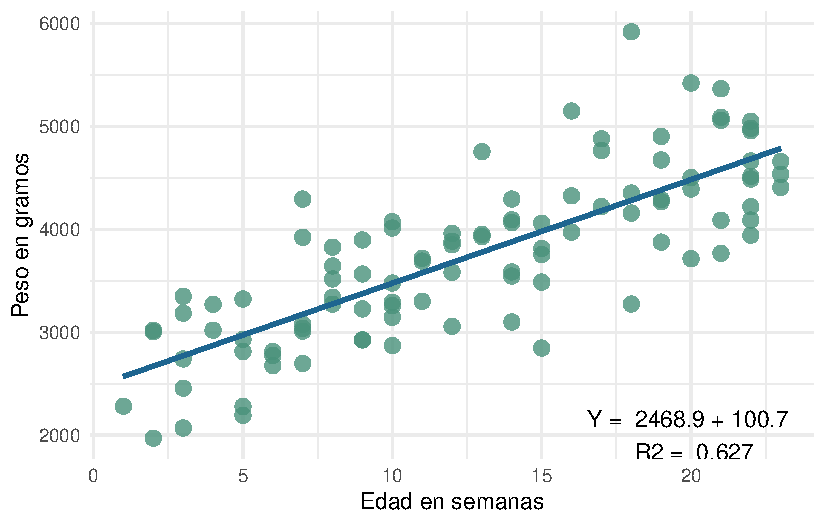
\includegraphics{index_files/figure-pdf/unnamed-chunk-5-1.pdf}

}

\caption{Gráfico 2. Función lineal. Edad y peso en 100 lactantes de sexo
femenino.}

\end{figure}%

La pendiente de la recta nos está indicando la magnitud y sentido de la
variación del peso en función de su edad para este grupo de lactantes.
En la ecuación, tanto la pendiente como el origen de la recta, se ponen
de manifiesto mediante los coeficientes. Un poco más adelante veremos
cómo se calculan y cómo se interpretan.

\begin{tcolorbox}[enhanced jigsaw, toptitle=1mm, colbacktitle=quarto-callout-tip-color!10!white, opacitybacktitle=0.6, leftrule=.75mm, rightrule=.15mm, title=\textcolor{quarto-callout-tip-color}{\faLightbulb}\hspace{0.5em}{Nota}, colframe=quarto-callout-tip-color-frame, breakable, coltitle=black, bottomrule=.15mm, opacityback=0, left=2mm, titlerule=0mm, bottomtitle=1mm, toprule=.15mm, colback=white, arc=.35mm]

El coeficiente de correlación (\emph{r} de Pearson) nos señala la fuerza
y el sentido (según su signo sea + o -) de esta relación lineal.

\end{tcolorbox}

\subsection{Modelos de Regresión}\label{modelos-de-regresiuxf3n}

Uno de los propósitos de los modelos en estadística es intentar explicar
la realidad de la manera más ``simple'' posible (lo cual no es sinónimo
de fácil!), desde su esencia, dejando de lado los elementos que podrían
cambiar en distintos momentos (o sea la variabilidad del fenómeno, que
algunos autores lo comparan con ``el ruido''). Existen algunos eventos
en la naturaleza que podemos explicar con total exactitud si conocemos
algunos datos, por ejemplo el volumen de un cubo. Con respecto a la
caída de un objeto, podríamos predecir con un margen de error casi nulo
su velocidad y su trayecto. Los modelos que explican estos fenómenos se
llaman ``modelos deterministas''. Sin embargo cuando queremos entender
la realidad que nos rodea la situación se complica, debido a que
aparecen otros factores que provocan que el valor de la variable
dependiente no pueda ser explicado o predicho completamente por la/s
otra/s variable/s. Los modelos que incorporan el concepto de ``error''
se denominan ``modelos probabilísticos'' y constituyen la mayoría de los
modelos que se abordan desde la estadística, que también se denominan
\emph{``modelos de regresión''}.

\begin{tcolorbox}[enhanced jigsaw, toptitle=1mm, colbacktitle=quarto-callout-tip-color!10!white, opacitybacktitle=0.6, leftrule=.75mm, rightrule=.15mm, title=\textcolor{quarto-callout-tip-color}{\faLightbulb}\hspace{0.5em}{Nota}, colframe=quarto-callout-tip-color-frame, breakable, coltitle=black, bottomrule=.15mm, opacityback=0, left=2mm, titlerule=0mm, bottomtitle=1mm, toprule=.15mm, colback=white, arc=.35mm]

la principal fuente del ``error'' se debe a la variabilidad entre
individuos propia de la naturaleza (por eso se denomina error
aleatorio). Puede haber otras fuentes de error, incluso no detectadas (y
que deben ser tenidas en cuenta), como pueden ser errores en la
medición, calibración o incluso por mala elección del método.

\end{tcolorbox}

Un modelo de regresión contiene una función que ``une'' a la variable
\(Y\) (independiente) con \(X\) (dependiente) y el \emph{``error
aleatorio''} (también llamado residuo o error residual). Esta función
puede ser lineal o no lineal según la naturaleza y distribución de la
variable independiente. El componente sistemático de la regresión es
esta función que deseamos ``modelar''.

El componente aleatorio es esa parte de la variación de \(Y\) que no
puede ser totalmente explicada por la variación de la/s variable/s
independiente/s. En algunos casos el error tendrá valor positivo y en
otros tendrá valor negativo. El promedio del error es igual a 0.

\[
Y = \underbrace{\beta_0 + \beta_1 X_1}_{Componente \: sistemático} + \underbrace{\epsilon}_{Componente \: aleatorio}
\]

Una vez que logremos establecer esta función estaremos en condiciones
de:

\begin{itemize}
\item
  Saber cómo se comporta la variable respuesta \(Y\) en función de la/s
  variable/s independientes.
\item
  Estimar o predecir el valor de \(Y\) para determinados valores de
  \(X\)
\item
  Calcular el intervalo de confianza para estas predicciones
\end{itemize}

Vamos a volver al ejemplo del peso en niñas menores de 6 meses, donde
habíamos trazado una recta que nos ilustraba la relación lineal del peso
en función de la edad.

Según el modelo estadístico para la función lineal de \(Y\) según \(X\):

\[Y(X) =  \beta_0 + \beta_1 + X_1\]

Hemos ajustado un modelo cuyos parámetros son:

\[\hat{y} = b_0 + b_1X_1\] \(b_1\) nos está indicando cuánto se modifica
\(\hat{y}\) por \textbf{cada unidad} de aumento de \(X_1\).

\[\hat{y} = 2468,9 + 100,7 \: edad \: (en \: semanas) \] Se interpreta
que por cada semana este grupo de lactantes ha aumentado en promedio 100
grs.

Cada 1 mes (4 semanas) aumentan una media de 400 grs.

Podemos observar que hay una relación lineal y que esta relación no es
perfecta. Existe cierta dispersión entre los puntos sugiriendo que
alguna variación en el peso no se asocia con un incremento de la edad
(por ejemplo dos lactantes de 15 semanas. Tienen la misma edad y 1.600
grs de diferencia. Cabría preguntarse si esas niñas que se ``alejan''
tanto de la recta de regresión no tienen algún antecedente distinto del
resto). Más adelante veremos cómo se interpretan esas diferentes
distancias entre las observaciones y la recta de regresión.

Ahora vamos a concentrarnos en la relación entre la varianza de la
muestra, a través del desvío estándar (\(ds = \sqrt{varianza}\)) y la
magnitud de la asociación. Se muestran 4 ejemplos en los cuáles se fue
aumentando progresivamente el desvío estándar de los datos. Observen
cómo a medida que aumenta la variabilidad entre los individuos va
disminuyendo el coeficiente de correlación y el coeficiente \(b_1\)
(pendiente de la recta)

\begin{center}
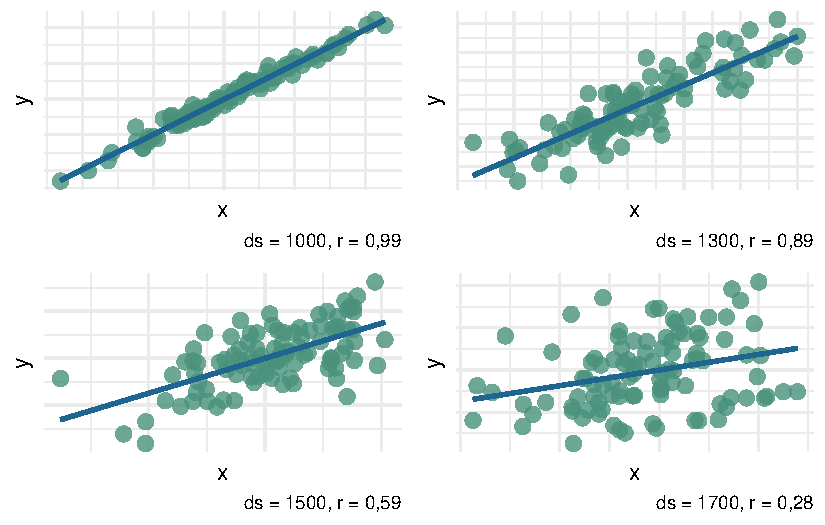
\includegraphics{index_files/figure-pdf/unnamed-chunk-6-1.pdf}
\end{center}

Podemos observar que cuanto mayor es la varianza en una muestra:

\begin{itemize}
\item
  Mayor es la variabilidad de \(y\) en torno a la recta de regresión
\item
  Mayor es la imprecisión asociada a la estimativa de los parámetros de
  regresión
\end{itemize}

\subsection{Modelo de Regresión:
Presupuestos}\label{modelo-de-regresiuxf3n-presupuestos}

Cuando planeamos realizar un análisis de regresión con un conjunto de
datos es necesario saber que para que podamos plantearlo adecuadamente
deben cumplirse ciertas condiciones, que llamaremos Presupuestos del
modelo:

\begin{enumerate}
\def\labelenumi{\arabic{enumi}.}
\tightlist
\item
  Independencia: los valores de \(y\) deben ser independientes unos de
  otros
\item
  Linealidad: la relación entre \(x\) e \(y\) debe ser una función
  lineal
\item
  Homocedasticidad: la varianza de \(y\) debe mantenerse constante para
  los distintos valores de \(x\)
\item
  Normalidad: \(y\) debe tener una distribución normal
\end{enumerate}

\textbf{¿Cómo se obtiene la recta de regresión? ¿Cómo se calculan los
coeficientes de la regresión?}

Volviendo al ejemplo del peso según edad en niñas menores de 6 meses la
idea es encontrar una función lineal (que gráficamente es una recta) que
aplicada a los valores de \(x\) nos permita aproximar los valores de
\(y\). La ecuación de la recta que describe la relación entre \(x\) e
\(y\):

\[\hat{y} = b_0 + b_1x\]

Por muy bueno que sea el modelo de regresión \(y\) e \(\hat{y}\) rara
vez coincidirán.

Entonces podríamos pensar que la mejor recta que permita predecir (o
aproximar) los valores de \(y\) en función de \(x\) es aquella que
minimice estos errores residuales (que algunos serán en más y otros
serán en menos).

Gráficamente:

\begin{center}
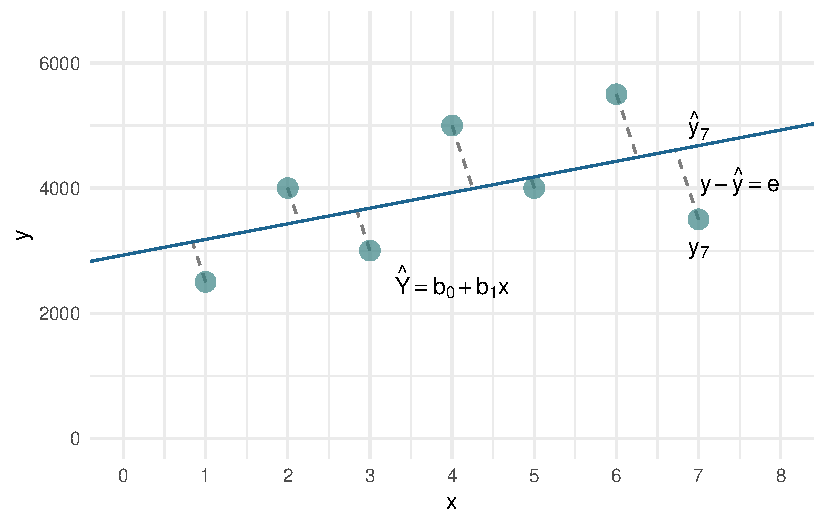
\includegraphics{index_files/figure-pdf/unnamed-chunk-7-1.pdf}
\end{center}

Donde:

\(\hat{y}\): es la ecuación de la ``mejor'' recta que puede trazarse
entre estos puntos

\(b_0\): ordenada al origen o constante, también llamada alfa. Es el
punto donde la recta de regresión corta al eje de ordenadas.

\(b_1\): pendiente de la recta (Un poco más adelante veremos cuál es la
interpretación de estos coeficientes)

Consideremos qué pasa en el caso de la niña 7. Veamos las distancias
para este punto.

\(y_7\): es el valor ``real'' del peso de la niña 7

\(\hat{y}_7\): es el valor estimado de \(y\) que obtendremos a través de
la regresión

\(y – \hat{y} = e\) (residuo o error residual) es el desvío de \(y\) del
valor ajustado \(\hat{y}\) en la ecuación de la regresión estimada

Para poder operar con el valor de estos errores (ya que algunos tendrán
valor positivo y otros valor negativo) se los eleva al cuadrado. Esta
técnica se denomina \textbf{``método de los mínimos cuadrados''} y
consiste en adoptar como estimativas de los parámetros de la regresión
(o sea los coeficientes \(b_0\) y \(b_1\) y por ende la recta de
regresión) los valores que minimizan la suma de los cuadrados de los
residuos o error (\textbf{SCE}) para todas las observaciones de \(y\).
Lo podemos expresar así:

\[SCE = \sum{\hat{e}^2} = \sum{(y-\hat{y})^2} \]

Sabíamos que \(\hat{y} = b_0 + b_1x\)

Entonces si reemplazamos:

\[SCE = \sum_{i=1}^{i=n} (y_i-\hat{y}_i)^2 =  \sum_{i=1}^{i=n}(y_i-(\hat{\beta}_0 + \hat{\beta}_1x_1))^2\]

Es posible obtener los estimadores \(\beta_1\) y \(\beta_0\).

\[\hat{\beta}_1 = \frac{\sum_{i=1}^{n}(x_i - \bar{x})(y_i - \bar{y})}{\sum_{i=1}^{n}(x_i-\bar{x})^2} = \frac{S_{xy}}{S_{xx}}  \]

Otra fórmula para \(\beta_1\):

\[\hat{\beta}_1 = \frac{\sum x_iy_i-\frac{\sum x_i \sum y_i}{n}}{\sum x_i^2 - \frac{(\sum x_i)^2}{n}} \]

\[\hat{\beta}_0 = \bar{y} - \beta_1\bar{x}  \]

El método de los mínimos cuadrados fue creado por \emph{Johann Carl
Friedrich Gauss} (1777-1855). Tiene además la ventaja que el promedio de
los errores residuales = 0 y que para cada estimación, la varianza del
error es mínima.

\textbf{Test de hipótesis para} \(\beta_1\) e Intervalo de Confianza
95\%

Como siempre que trabajamos con una muestra, será necesario aplicar los
procesos de inferencia. Es por eso que los softwares ofrecen un test de
hipótesis para el coeficiente.

La hipótesis nula podría entenderse como que \(x\) no logra explicar la
variación de \(y\) (entonces la pendiente de la recta sería nula)

\[H_0: \beta_1 = 0 \]

Al calcular el modelo de regresión, todos los softwares estiman el
coeficiente y el error estándar del mismo (se) y testean el coeficiente.

\textbf{Bondad de ajuste}

Hasta ahora hemos aprendido a explicar la variación de \(y\) según la
variación de \(x\) mediante un modelo en donde las desviaciones entre el
valor observado (``real'') y el estimado (``modelo de regresión'') son
las menores posibles.

Ahora debemos saber, según los datos que tenemos, cuán bueno es el
modelo que ajustamos (qué capacidad tiene de explicar la variabilidad de
\(y\) o, si lo quiero utilizar para realizar una predicción, cuánto se
alejará mi valor estimado del verdadero, ``real'' valor de \(y\)). Esta
evaluación la realizaremos mediante la descomposición de la varianza del
modelo. Por definición la varianza o variabilidad total es la sumatoria
de la diferencia entre cada valor de \(y\) con el promedio de \(y\)
(elevado al cuadrado ya que hay valores negativos y positivos que si los
sumamos se anularían).

La variabilidad total del modelo es la suma entre la variabilidad que
logró explicar la regresión y la variabilidad residual.

\[\sum (y_i-\bar{y})^2 = \sum (\hat{y}-\bar{y})^2 + \sum (y_i -\hat{y}_i)^2 \]

\[\frac{Suma \; de \; cuadrados}{totales \; (SCT)} \; \frac{Suma \; de \; cuadrados}{de \; la \; regresion \; (SCR)} \; \frac{Suma \; de \; cuadrados}{residuales \; (SCE)}\]

Cuanto mayor sea la variabilidad que logre explicar la regresión en
relación a los residuos, tanto mejor será el modelo. Este es el
fundamento para el cálculo del coeficiente de determinación (\(R^2\))

\[R^2 = \frac{SCR}{SCT} = 1 - \frac{SCE}{SCT}\]

\(R^2\) expresa la proporción de la variación total que logra explicar
el modelo de regresión. Su valor oscila entre 0 y 1, es una cantidad
adimensional.

\begin{itemize}
\item
  Cuando el ajuste es bueno \(R^2\) será cercano a 1, cuando el ajuste
  es malo \(R^2\) será cercano a 0.
\item
  En la Regresión lineal simple el coeficiente de determinación
  (\(R^2\)) es igual al \(r\) de Pearson elevado al cuadrado.
\end{itemize}

Para visualizar simulaciones al respecto pueden visitar
\href{https://seeing-theory.brown.edu/regression-analysis/es.html\#section1}{Viendo
la teoría. Una introducción visual a probabilidad y estadística}

\subsection{Ejemplo práctico en lenguaje
R}\label{ejemplo-pruxe1ctico-en-lenguaje-r}

Para llevar a cabo el análisis en R y presentar las funciones y paquetes
que nos pueden ayudar en la tarea vamos a trabajar con un set de datos
llamado \texttt{cancer\_rls} que contiene información sobre la tasa de
mortalidad por cáncer cada 100.000 habitantes de distintos condados de
Estados Unidos.

El dataset contiene datos agregados sobre la tasa de mortalidad por
cáncer, el porcentaje de personas con cobertura pública de salud, el
porcentaje de personas bajo la línea de pobreza y la mediana de edad.
Para el ejemplo de regresión linear simple, evaluaremos la asociación
entre cobertura pública de salud y mortalidad por cáncer.

\begin{Shaded}
\begin{Highlighting}[]
\DocumentationTok{\#\#\# Carga paquetes}
\CommentTok{\# tablas salida del modelo}
\FunctionTok{library}\NormalTok{(gtsummary)}

\CommentTok{\# chequeo de supuestos y análisis de residuales}
\FunctionTok{library}\NormalTok{(performance)}
\FunctionTok{library}\NormalTok{(lmtest) }
\FunctionTok{library}\NormalTok{(nortest)}

\CommentTok{\# manejo de datos}
\FunctionTok{library}\NormalTok{(tidyverse) }


\DocumentationTok{\#\#\# Carga datos}
\NormalTok{datos }\OtherTok{\textless{}{-}} \FunctionTok{read\_csv2}\NormalTok{(}\StringTok{"cancer\_rls.txt"}\NormalTok{)}
\end{Highlighting}
\end{Shaded}

La estructura de la tabla es:

\begin{Shaded}
\begin{Highlighting}[]
\FunctionTok{glimpse}\NormalTok{(datos)}
\end{Highlighting}
\end{Shaded}

\begin{verbatim}
Rows: 236
Columns: 4
$ target_death_rate   <dbl> 179.8, 217.7, 195.2, 205.2, 173.1, 200.3, 149.0, 1~
$ pct_public_coverage <dbl> 28.8, 45.6, 48.0, 27.3, 41.2, 47.0, 30.5, 46.6, 42~
$ poverty_percent     <dbl> 15.0, 24.6, 27.5, 10.7, 15.8, 23.6, 7.9, 23.3, 28.~
$ median_age          <dbl> 39.1, 39.6, 45.0, 41.0, 32.2, 40.8, 45.4, 56.5, 37~
\end{verbatim}

La variable dependiente es la tasa de mortalidad
(\texttt{target\_death\_rate}) y la independiente la mediana de edad
(\texttt{median\_age}).

\subsubsection{Diagrama de dispersión}\label{diagrama-de-dispersiuxf3n}

Para dibujar gráficos de dispersión podemos utilizar funciones del
paquete \texttt{ggplot2}.

\begin{Shaded}
\begin{Highlighting}[]
\NormalTok{datos }\SpecialCharTok{\%\textgreater{}\%} 
  
  \FunctionTok{ggplot}\NormalTok{(}\FunctionTok{aes}\NormalTok{(}\AttributeTok{x =}\NormalTok{ median\_age, }\AttributeTok{y =}\NormalTok{ target\_death\_rate)) }\SpecialCharTok{+}
  
  \CommentTok{\# gráfico de dispersión}
  \FunctionTok{geom\_point}\NormalTok{(}\AttributeTok{color =} \StringTok{"\#49917A"}\NormalTok{) }\SpecialCharTok{+} 
  
  \CommentTok{\# modifico color de fondo}
  \FunctionTok{theme\_minimal}\NormalTok{()}
\end{Highlighting}
\end{Shaded}

\begin{center}
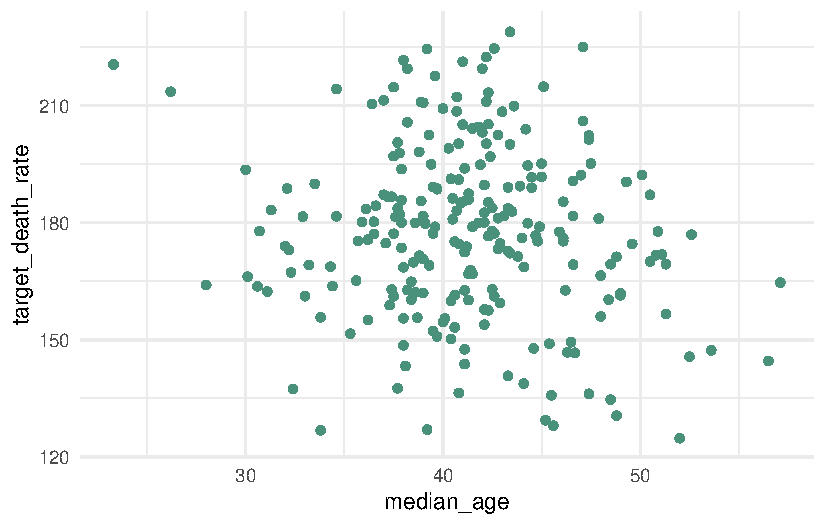
\includegraphics{index_files/figure-pdf/unnamed-chunk-10-1.pdf}
\end{center}

En todos los casos, lo que observamos en el gráfico es una clara
relación inversa entre las variables, dado que las ciudades que tienen
altos valores en porcentajes de ciclistas tiene bajos valores en
porcentajes de cardiopatías y viceversa.

\subsubsection{Correlación}\label{correlaciuxf3n}

La función \texttt{cor()} estima la correlación entre dos variables. El
método predeterminado devuelve la correlación de Pearson, pero puede
modificarse el argumento \texttt{method} para obtener la correlación de
Kendall o Spearman.

\begin{Shaded}
\begin{Highlighting}[]
\FunctionTok{cor}\NormalTok{(datos}\SpecialCharTok{$}\NormalTok{median\_age, datos}\SpecialCharTok{$}\NormalTok{target\_death\_rate,}
    \AttributeTok{method =} \StringTok{"pearson"}\NormalTok{)}
\end{Highlighting}
\end{Shaded}

\begin{verbatim}
[1] -0.1346534
\end{verbatim}

El valor es negativo, lo que confirma lo observado en la nube de puntos
anterior.

\textbf{Significación de la correlación}

Hasta ahora obtuvimos dos elementos de la correlación, la magnitud y el
signo.

Para poder descartar que esta \textbf{correlación negativa} se debe al
azar, debemos calcular su significancia.

La función \texttt{cor.test()} determina si la prueba de correlación de
Pearson calculada es significativa y lo realiza mediante el estadístico
\(t\) de Student.

\begin{Shaded}
\begin{Highlighting}[]
\FunctionTok{cor.test}\NormalTok{(datos}\SpecialCharTok{$}\NormalTok{median\_age, datos}\SpecialCharTok{$}\NormalTok{target\_death\_rate)}
\end{Highlighting}
\end{Shaded}

\begin{verbatim}

    Pearson's product-moment correlation

data:  datos$median_age and datos$target_death_rate
t = -2.0787, df = 234, p-value = 0.03873
alternative hypothesis: true correlation is not equal to 0
95 percent confidence interval:
 -0.25791890 -0.00707458
sample estimates:
       cor 
-0.1346534 
\end{verbatim}

Los resultados de la función son:

\begin{itemize}
\tightlist
\item
  El valor del estadístico \(t\)
\item
  El valor de \(p\) para el estadístico
\item
  El valor de la correlación de Pearson
\item
  Los intervalos de confianza para la correlación
\end{itemize}

Los argumentos predeterminados para la función \texttt{cor.test()} son:

\texttt{alternative\ =\ "two.sided"} - indica la hipotesis alternativa,
también puede ser \texttt{"greater"} para asociación positiva,
\texttt{"less"} para asociación negativa.

\texttt{conf.level\ =\ 0.95} - determina el nivel de confianza (se puede
modificar).

\texttt{method\ =\ "pearson"} - especifíca el tipo de test de
correlación. También permite \texttt{"kendall"} o \texttt{"spearman".}

El \emph{p}-valor de la correlación para este ejemplo es menor a 0,05
(\emph{p}-value: 0.0387318), por lo tanto significativa.

\subsubsection{Presupuestos}\label{presupuestos}

Anteriormente mencionamos que para dar por válidos, los modelos lineales
debían cumplir con cuatro presupuestos: independencia, linealidad,
homocedasticidad y normalidad.

Habitualmente la comprobación precisa de estos criterios se realiza con
los residuos del modelo al finalizar el proceso, pero también nos
podemos adelantar efectuando un análisis previo de los datos de forma
similar a lo realizado en ANOVA.

La independencia, también conocida como no autocorrelación, pueden
afirmarse de forma general, a partir del conocimiento previo de la
fuente de los datos y su forma de recolección, aunque siempre conviene
verificarla en los residuos.

La linealidad es producto de la relación entre las variables
cardiopatias y ciclistas, que confirmamos mediante el diagrama de
dispersión y la \(r\) de Pearson significativa.

La homocedasticidad es conveniente definirla a partir del modelo
realizado, donde buscamos que la varianza de la gráfica de los residuos
sea aproximadamente constante a lo largo del eje x. También se puede
probar mediante contraste de hipótesis (test de Breusch-Pagan)

Finalmente para la normalidad utilizamos el mismo análisis previo visto
en la unidad anterior (ver
\href{https://cballejo.github.io/R_Epi_Avanzada/Unidad2/Anova/}{ANOVA -
Unidad 2})

\begin{Shaded}
\begin{Highlighting}[]
\DocumentationTok{\#\# Test normalidad}
\FunctionTok{lillie.test}\NormalTok{(datos}\SpecialCharTok{$}\NormalTok{target\_death\_rate)}
\end{Highlighting}
\end{Shaded}

\begin{verbatim}

    Lilliefors (Kolmogorov-Smirnov) normality test

data:  datos$target_death_rate
D = 0.030015, p-value = 0.8706
\end{verbatim}

\begin{Shaded}
\begin{Highlighting}[]
\DocumentationTok{\#\# QQplot}
\NormalTok{datos }\SpecialCharTok{\%\textgreater{}\%} 
  \FunctionTok{ggplot}\NormalTok{(}\AttributeTok{mapping =} \FunctionTok{aes}\NormalTok{(}\AttributeTok{sample =}\NormalTok{ target\_death\_rate)) }\SpecialCharTok{+}
  
  \CommentTok{\# añade qqplot}
  \FunctionTok{stat\_qq}\NormalTok{() }\SpecialCharTok{+}
  \FunctionTok{stat\_qq\_line}\NormalTok{() }\SpecialCharTok{+}
  
  \CommentTok{\# cambia nombres de los ejes X e Y}
  \FunctionTok{labs}\NormalTok{(}\AttributeTok{title =} \StringTok{"QQplot"}\NormalTok{, }
       \AttributeTok{x =} \StringTok{"Theoretical Quantiles"}\NormalTok{, }
       \AttributeTok{y =} \StringTok{"Sample Quantiles"}\NormalTok{) }\SpecialCharTok{+}
  
  \CommentTok{\# modifico color de fondo}
  \FunctionTok{theme\_minimal}\NormalTok{()}
\end{Highlighting}
\end{Shaded}

\begin{center}
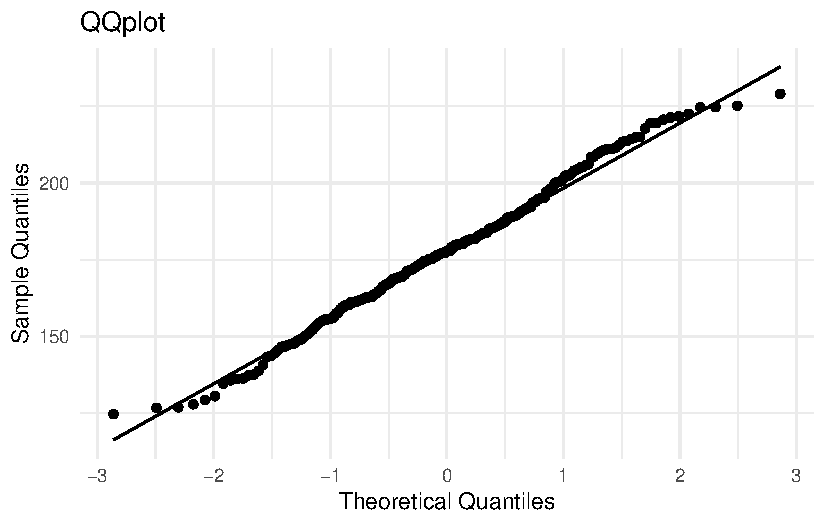
\includegraphics{index_files/figure-pdf/unnamed-chunk-13-1.pdf}
\end{center}

Tanto el test de hipótesis como los gráficos de cuantiles nos informan
que las distribuciones de la variable dependiente cumple con el criterio
de ``normalidad''.

\subsubsection{Modelo lineal simple}\label{modelo-lineal-simple}

Para construir modelos de regresión utilizamos en los argumentos el
formato fórmula. Esto significa especificar primero el nombre de la
variable dependiente y luego la variable independiente.

La estructura sintáctica es:

\begin{quote}
variable\_dependiente \textasciitilde{} variable\_independiente
\end{quote}

La función que recibe esta estructura tipo fórmula es \texttt{lm()}
cuyas letras vienen de ``linear models'' (modelos lineales).

\begin{Shaded}
\begin{Highlighting}[]
\FunctionTok{lm}\NormalTok{(target\_death\_rate }\SpecialCharTok{\textasciitilde{}}\NormalTok{ median\_age, }\AttributeTok{data =}\NormalTok{ datos)}
\end{Highlighting}
\end{Shaded}

\begin{verbatim}

Call:
lm(formula = target_death_rate ~ median_age, data = datos)

Coefficients:
(Intercept)   median_age  
   201.3229      -0.5682  
\end{verbatim}

La función muestra resultados básicos, tales como la relación entre las
variables que son parte del modelo y los coeficientes.

\textbf{Intercept} es el valor de \texttt{median\_age} cuando
\texttt{target\_death\_rate} vale cero (Ordenada en el origen) y el
coeficiente de \texttt{median\_age}representa la pendiente de la recta.

Estos resultados obtenidos y aplicados en la fórmula del modelo simple
quedarían así:

\[\operatorname{target death rate} = \alpha + \beta_{1}(\operatorname{median age}) + \epsilon \]

\[
\operatorname{target death rate} = 201.3229 + -0.5682*\operatorname{median age} + \epsilon
\]

Habitualmente \texttt{lm()} suele asignarse a un objeto de regresión
para que contenga todos los resultados producto del ajuste.

\begin{Shaded}
\begin{Highlighting}[]
\NormalTok{modelo }\OtherTok{\textless{}{-}} \FunctionTok{lm}\NormalTok{(target\_death\_rate }\SpecialCharTok{\textasciitilde{}}\NormalTok{ median\_age, }\AttributeTok{data =}\NormalTok{ datos)}
\end{Highlighting}
\end{Shaded}

Los resultados se almacenan en forma de lista y sus componentes pueden
ser llamados en resúmenes más completos, mediante \texttt{summary()} o
por separado, por ejemplo para evaluar los residuos.

\begin{Shaded}
\begin{Highlighting}[]
\FunctionTok{summary}\NormalTok{(modelo)}
\end{Highlighting}
\end{Shaded}

\begin{verbatim}

Call:
lm(formula = target_death_rate ~ median_age, data = datos)

Residuals:
    Min      1Q  Median      3Q     Max 
-55.317 -15.899   0.176  14.845  52.338 

Coefficients:
            Estimate Std. Error t value Pr(>|t|)    
(Intercept) 201.3229    11.3689  17.708   <2e-16 ***
median_age   -0.5682     0.2734  -2.079   0.0387 *  
---
Signif. codes:  0 '***' 0.001 '**' 0.01 '*' 0.05 '.' 0.1 ' ' 1

Residual standard error: 21.96 on 234 degrees of freedom
Multiple R-squared:  0.01813,   Adjusted R-squared:  0.01394 
F-statistic: 4.321 on 1 and 234 DF,  p-value: 0.03873
\end{verbatim}

Con \texttt{summary()} observamos que los resultados son numerosos y
comprenden a:

\textbf{Call}: formula del modelo

\textbf{Residuals}: distribución de los residuos (mediana, mínimo,
máximo y percentilos 25-75)

\textbf{Coefficients}: valores del intercepto y de la pendiente. Además
se agregan los errores estandar y el estadístico \(t\) con el
\emph{p}-valor de probabilidad dada la hipótesis nula que los
coeficientes sean iguales a cero. (Lo que se pretende mediante estos
contrastes es determinar si los efectos de la constante intercepto y de
la variable independiente son realmente importantes para explicar la
variable dependiente o si, por el contario, pueden considerarse nulos.)

\textbf{Residual standard error}: Error estándar de los residuos con sus
grados de libertad

\textbf{Multiple R-squared}: Coeficiente de determinación \(R^2\)

\textbf{Adjusted R-squared}: Coeficiente \(R^2\) ajustado

\textbf{F-statistic}: estadístico \(F\) sobre la hipótesis nula que el
cociente entre la varianza de la ecuación de regresión y la varianza de
los residuos es igual a 1.

\textbf{p-value}: p-valor del estadistico \(F\).

Como elemento extra, notese que la salida en R tiene unos códigos que
ayudan a realizar la lectura de la significación de los coeficientes.
Funciona mediante el uso de asteriscos (*) al extremo derecho de cada
parámetro calculado.

Debajo de la tabla de coeficientes se encuentra la referencia del
significado de los códigos, que van desde el 0 hasta el 1 como posible
resultado del valor de probabilidad, y donde:

\global\setlength{\Oldarrayrulewidth}{\arrayrulewidth}

\global\setlength{\Oldtabcolsep}{\tabcolsep}

\setlength{\tabcolsep}{2pt}

\renewcommand*{\arraystretch}{1.5}



\providecommand{\ascline}[3]{\noalign{\global\arrayrulewidth #1}\arrayrulecolor[HTML]{#2}\cline{#3}}

\begin{longtable*}[c]{cc}



\ascline{1.5pt}{666666}{1-2}

\multicolumn{1}{>{}l}{\textcolor[HTML]{000000}{\fontsize{12}{12}\selectfont{\global\setmainfont{Calibri}{\textbf{Código}}}}} & \multicolumn{1}{>{}l}{\textcolor[HTML]{000000}{\fontsize{12}{12}\selectfont{\global\setmainfont{Calibri}{\textbf{Rango}}}}} \\

\ascline{1.5pt}{666666}{1-2}\endfirsthead 

\ascline{1.5pt}{666666}{1-2}

\multicolumn{1}{>{}l}{\textcolor[HTML]{000000}{\fontsize{12}{12}\selectfont{\global\setmainfont{Calibri}{\textbf{Código}}}}} & \multicolumn{1}{>{}l}{\textcolor[HTML]{000000}{\fontsize{12}{12}\selectfont{\global\setmainfont{Calibri}{\textbf{Rango}}}}} \\

\ascline{1.5pt}{666666}{1-2}\endhead



\multicolumn{1}{>{}l}{\textcolor[HTML]{000000}{\fontsize{12}{12}\selectfont{\global\setmainfont{Calibri}{***}}}} & \multicolumn{1}{>{}l}{\textcolor[HTML]{000000}{\fontsize{12}{12}\selectfont{\global\setmainfont{Calibri}{0\ a\ 0,001}}}} \\





\multicolumn{1}{>{}l}{\textcolor[HTML]{000000}{\fontsize{12}{12}\selectfont{\global\setmainfont{Calibri}{**}}}} & \multicolumn{1}{>{}l}{\textcolor[HTML]{000000}{\fontsize{12}{12}\selectfont{\global\setmainfont{Calibri}{0,001\ a\ 0,01}}}} \\





\multicolumn{1}{>{}l}{\textcolor[HTML]{000000}{\fontsize{12}{12}\selectfont{\global\setmainfont{Calibri}{*}}}} & \multicolumn{1}{>{}l}{\textcolor[HTML]{000000}{\fontsize{12}{12}\selectfont{\global\setmainfont{Calibri}{0,01\ a\ 0,05}}}} \\





\multicolumn{1}{>{}l}{\textcolor[HTML]{000000}{\fontsize{12}{12}\selectfont{\global\setmainfont{Calibri}{.}}}} & \multicolumn{1}{>{}l}{\textcolor[HTML]{000000}{\fontsize{12}{12}\selectfont{\global\setmainfont{Calibri}{0,05\ a\ 0,1}}}} \\





\multicolumn{1}{>{}l}{\textcolor[HTML]{000000}{\fontsize{12}{12}\selectfont{\global\setmainfont{Calibri}{}}}} & \multicolumn{1}{>{}l}{\textcolor[HTML]{000000}{\fontsize{12}{12}\selectfont{\global\setmainfont{Calibri}{0,1\ a\ 1}}}} \\

\ascline{1.5pt}{666666}{1-2}



\end{longtable*}



\arrayrulecolor[HTML]{000000}

\global\setlength{\arrayrulewidth}{\Oldarrayrulewidth}

\global\setlength{\tabcolsep}{\Oldtabcolsep}

\renewcommand*{\arraystretch}{1}

\paragraph{Estructura del objeto resultado de
regresión}\label{estructura-del-objeto-resultado-de-regresiuxf3n}

Todos los ajustes de modelos lineales que produce la función
\texttt{lm()} tienen la forma de una lista de 12 componentes.

La manera de conocer su clase es \texttt{class()} y su estructura
mediante \texttt{str()}

\begin{Shaded}
\begin{Highlighting}[]
\FunctionTok{class}\NormalTok{(modelo)}
\FunctionTok{str}\NormalTok{(modelo)}
\end{Highlighting}
\end{Shaded}

La clase de este tipo (clase base = lista) es ``lm'' y de todos estos
componentes, los más relevantes son:

\textbf{coefficients}

Es un vector con dos valores. El intercepto y la pendiente de la recta.

Lo podemos llamar desde el objeto:

\begin{Shaded}
\begin{Highlighting}[]
\NormalTok{modelo}\SpecialCharTok{$}\NormalTok{coefficients}
\end{Highlighting}
\end{Shaded}

\begin{verbatim}
(Intercept)  median_age 
201.3229258  -0.5682328 
\end{verbatim}

O bien utilizar la función \texttt{coef()}

\begin{Shaded}
\begin{Highlighting}[]
\FunctionTok{coef}\NormalTok{(modelo)}
\end{Highlighting}
\end{Shaded}

\begin{verbatim}
(Intercept)  median_age 
201.3229258  -0.5682328 
\end{verbatim}

La función \texttt{tbl\_regression()} del paquete \texttt{gtsummary}
también nos permite explorar los coeficientes del modelo, ajustando el
nivel de confianza con el argumento \texttt{conf.level} y mostrando u
ocultando el intercepto con el argumento \texttt{intercept}.

\begin{Shaded}
\begin{Highlighting}[]
\FunctionTok{tbl\_regression}\NormalTok{(modelo, }
               \AttributeTok{intercept =}\NormalTok{ T, }
               \AttributeTok{conf.level =}\NormalTok{ .}\DecValTok{95}\NormalTok{)}
\end{Highlighting}
\end{Shaded}

\begin{longtable}[]{@{}lccc@{}}
\toprule\noalign{}
\textbf{Characteristic} & \textbf{Beta} & \textbf{95\% CI} &
\textbf{p-value} \\
\midrule\noalign{}
\endhead
\bottomrule\noalign{}
\endlastfoot
(Intercept) & 201 & 179, 224 & \textless0.001 \\
median\_age & -0.57 & -1.1, -0.03 & 0.039 \\
\end{longtable}

\textbf{residuals}

Los residuos o residuales para cada valor que surgen de la diferencia
entre los valores predictivos calculados por el modelo y los valores
reales.

Se visualizan desde el objeto resultado de la regresión:

\begin{Shaded}
\begin{Highlighting}[]
\NormalTok{modelo}\SpecialCharTok{$}\NormalTok{residuals}
\end{Highlighting}
\end{Shaded}

Usando la función \texttt{resid()}

\begin{Shaded}
\begin{Highlighting}[]
\FunctionTok{resid}\NormalTok{(modelo)}
\end{Highlighting}
\end{Shaded}

\textbf{fitted.values}

Los valores calculados por el modelo en base a los datos existentes en
la variable independiente.

Los encontramos en:

\begin{Shaded}
\begin{Highlighting}[]
\NormalTok{modelo}\SpecialCharTok{$}\NormalTok{fitted.values}
\end{Highlighting}
\end{Shaded}

También pueden ser vistos por medio de la función \texttt{fitted()}

\begin{Shaded}
\begin{Highlighting}[]
\FunctionTok{fitted}\NormalTok{(modelo)}
\end{Highlighting}
\end{Shaded}

Otra función interesante para el análisis del objeto de regresión es
\texttt{confint()} que calcula los intervalos de confianza de los
coeficientes o parámetros del modelo de regresión.

Para este modelo la línea de ejecución de la función es:

\begin{Shaded}
\begin{Highlighting}[]
\FunctionTok{confint}\NormalTok{(modelo)}
\end{Highlighting}
\end{Shaded}

\begin{verbatim}
                 2.5 %       97.5 %
(Intercept) 178.924420 223.72143175
median_age   -1.106785  -0.02968067
\end{verbatim}

Si agregamos la función \texttt{round()} podemos redondear los valores
con la cantidad de decimales que necesitemos.

\begin{Shaded}
\begin{Highlighting}[]
\DocumentationTok{\#\# redondeo con 2 decimales}
\FunctionTok{round}\NormalTok{(}\FunctionTok{confint}\NormalTok{(modelo),}\DecValTok{2}\NormalTok{)  }
\end{Highlighting}
\end{Shaded}

\begin{verbatim}
             2.5 % 97.5 %
(Intercept) 178.92 223.72
median_age   -1.11  -0.03
\end{verbatim}

En forma predeterminada los IC se calculan al 95\%, pero mediante el
argumento \texttt{level} podemos modificarlo, por ejemplo al 99\%:

\begin{Shaded}
\begin{Highlighting}[]
\FunctionTok{confint}\NormalTok{(modelo, }\AttributeTok{level =} \FloatTok{0.99}\NormalTok{)}
\end{Highlighting}
\end{Shaded}

\begin{verbatim}
                 0.5 %      99.5 %
(Intercept) 171.797830 230.8480220
median_age   -1.278138   0.1416719
\end{verbatim}

\subsubsection{Agregar la recta de regresión al diagrama de
dispersión}\label{agregar-la-recta-de-regresiuxf3n-al-diagrama-de-dispersiuxf3n}

Retomando la cuestión gráfica, podemos dibujar la recta de regresión
lineal sobre el diagrama de dispersión hecho con \texttt{ggplot2}
adicionando una capa más al gráfico mediante \texttt{geom\_smooth()} e
indicando \texttt{method\ =\ "lm"} como método. Además de la recta se
puede ver el IC (zona gris alrededor de ella).

\begin{Shaded}
\begin{Highlighting}[]
\NormalTok{datos }\SpecialCharTok{\%\textgreater{}\%} 
  \FunctionTok{ggplot}\NormalTok{(}\FunctionTok{aes}\NormalTok{(}\AttributeTok{x =}\NormalTok{ median\_age, }\AttributeTok{y =}\NormalTok{ target\_death\_rate)) }\SpecialCharTok{+}
  
 \CommentTok{\# diagrama de dispersión}
   \FunctionTok{geom\_point}\NormalTok{(}\AttributeTok{color =} \StringTok{"\#49917A"}\NormalTok{) }\SpecialCharTok{+}
  
  \CommentTok{\# añade línea de regresión}
  \FunctionTok{geom\_smooth}\NormalTok{(}\AttributeTok{method =} \StringTok{"lm"}\NormalTok{, }\AttributeTok{color =} \StringTok{"\#1E6590"}\NormalTok{) }\SpecialCharTok{+} 
  
  \CommentTok{\# cambia color de fondo}
  \FunctionTok{theme\_minimal}\NormalTok{()}
\end{Highlighting}
\end{Shaded}

\begin{center}
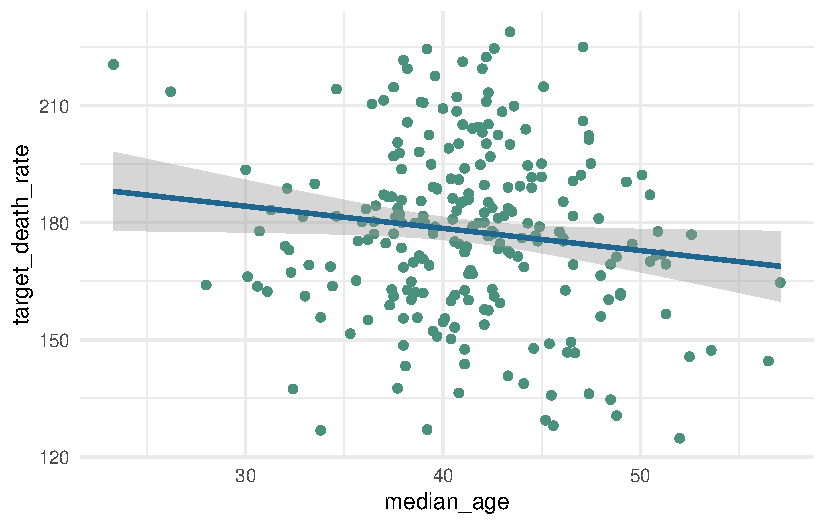
\includegraphics{index_files/figure-pdf/unnamed-chunk-29-1.pdf}
\end{center}

\subsubsection{Residuales}\label{residuales}

El residuo o residual de una estimación se define como la diferencia
entre el valor observado y el valor calculado por el modelo de
regresión.

A la hora de resumir el conjunto de residuales hay dos posibilidades:

\begin{itemize}
\item
  La sumatoria del valor absoluto de cada residual.
\item
  La sumatoria del cuadrado de cada residuo (RSS). Esta es la
  aproximación más empleada (mínimos cuadrados) ya que magnifica las
  desviaciones extremas.
\end{itemize}

En R vimos que estos residuos quedan almacenados dentro del objeto de
regresión y pueden ser llamados mediante la expresión
\texttt{nombre\_del\_objeto\_de\_regresion\$residuals}

Cuanto mayor es la sumatoria del cuadrado de los residuales menor la
precisión con la que el modelo puede predecir el valor de la variable
dependiente a partir de la variable predictora. Los residuales son muy
importantes puesto que en ellos se basan las diferentes medidas de la
bondad de ajuste del modelo y con ellos se determina el cumplimiento de
los supuestos de los modelos lineales.

Un análisis visual de estos residuos se puede obtener fácilmente
aplicando la función \texttt{plot()} al objeto de regresión modelado. La
salida presentará 4 gráficas automáticas.

\begin{Shaded}
\begin{Highlighting}[]
\FunctionTok{par}\NormalTok{(}\AttributeTok{mfrow =} \FunctionTok{c}\NormalTok{(}\DecValTok{2}\NormalTok{,}\DecValTok{2}\NormalTok{))}
\FunctionTok{plot}\NormalTok{(modelo)}
\end{Highlighting}
\end{Shaded}

\begin{center}
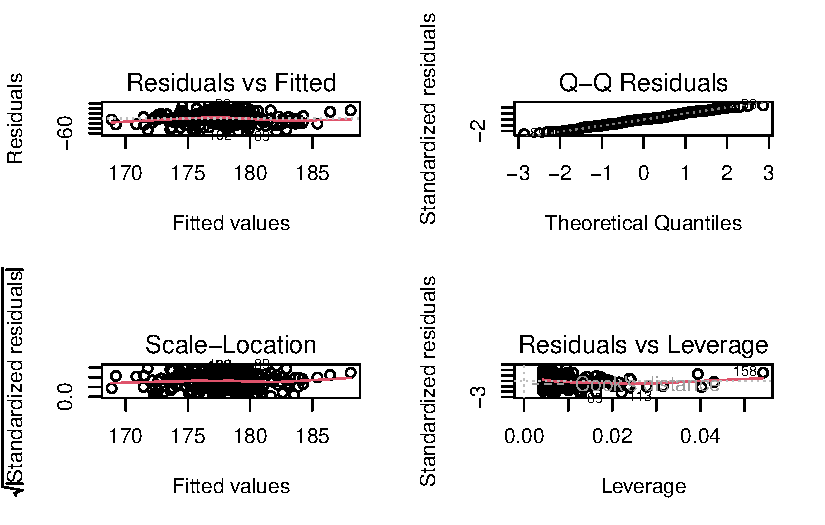
\includegraphics{index_files/figure-pdf/unnamed-chunk-30-1.pdf}
\end{center}

El gráfico \textbf{Residuals vs Fitted} (Residuales vs valores
ajustados) sirve para probar linealidad.

Se examina evaluando que la linea roja sea lo mas horizontal posible y
sin curvatura pronunciada. Si tuviera curvatura indicaría que el modelo
puede necesitar un término de ajuste no lineal (por ejemplo: cuadrático,
logarítmico, etc) o que hay una variable importante no incluida en el
modelo.

El siguiente gráfico \textbf{Normal Q-Q}, es el típico diagrama de
cuantiles para evaluar normalidad, donde los valores (puntos) deben
estar lo más cercanos de la linea diagonal. Las desviaciones
pronunciadas indican desajuste.

\textbf{Scale-Location} es útil para ver si los residuales se
distribuyen por igual a lo largo del rango de los predictores. Así es
como se puede verificar la suposición de igual varianza
(homocedasticidad).

Es bueno si vemos una línea aproximadamente horizontal con puntos de
distribución igualmente aleatorios.

Finalmente el cuarto diagrama \textbf{Residuals vs Leverage} nos ayuda a
encontrar valores influyentes.

Aunque los datos tengan valores extremos, es posible que no sean
influyentes para determinar una línea de regresión. Eso significa que
los resultados no serían muy diferentes si los incluyéramos o los
excluyéramos del análisis.

Pero existen otros valores que si pueden influir y en el gráfico
aparecen en las esquinas, fuera de unas líneas rojas entrecortadas que
determinan altas puntuaciones de distancia de Cook (medida muy utilizada
que combina, en un único valor, la magnitud del residual y el grado de
leverage).

Otra forma de evaluar gráficamente los supuestos del modelo es mediante
la función \texttt{check\_model()} del paquete \texttt{performance}:

\begin{Shaded}
\begin{Highlighting}[]
\FunctionTok{check\_model}\NormalTok{(modelo)}
\end{Highlighting}
\end{Shaded}

\begin{center}
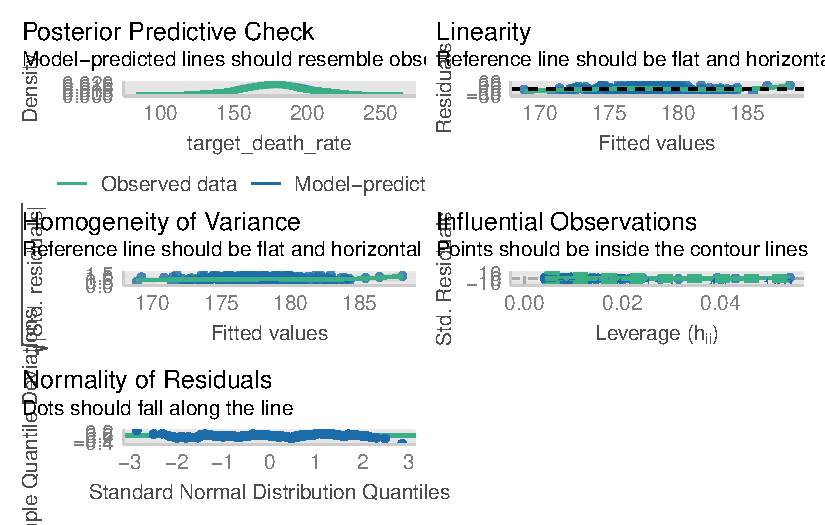
\includegraphics{index_files/figure-pdf/unnamed-chunk-31-1.pdf}
\end{center}

El argumento \texttt{check} nos permite seleccionar cuales gráficos de
residuales queremos visualizar (opciones:
\texttt{"all"},~\texttt{"vif"},~\texttt{"qq"},~\texttt{"normality"},~\texttt{"linearity"},~\texttt{"ncv"},~\texttt{"homogeneity"},~\texttt{"outliers"},~\texttt{"reqq"},~\texttt{"pp\_check"},~\texttt{"binned\_residuals"},~\texttt{"overdispersion"}).

\begin{Shaded}
\begin{Highlighting}[]
\FunctionTok{check\_model}\NormalTok{(modelo, }\AttributeTok{check =} \FunctionTok{c}\NormalTok{(}\StringTok{"normality"}\NormalTok{,}\StringTok{"qq"}\NormalTok{, }\StringTok{"linearity"}\NormalTok{,}
                              \StringTok{"homogeneity"}\NormalTok{, }\StringTok{"outliers"}\NormalTok{))}
\end{Highlighting}
\end{Shaded}

\begin{center}
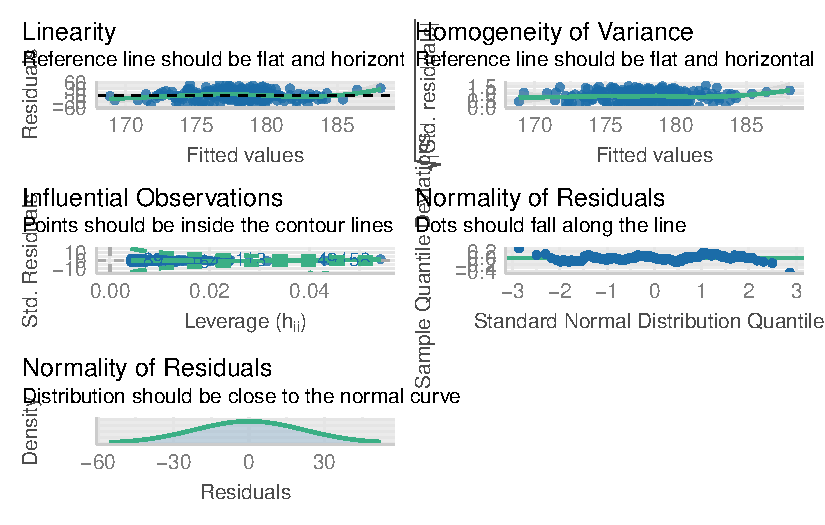
\includegraphics{index_files/figure-pdf/unnamed-chunk-32-1.pdf}
\end{center}

Además del análisis gráfico/visual de residuos se pueden aplicar test
analíticos.

\textbf{Linealidad}

El paquete \texttt{lmtest} implementa el \emph{Ramsey's RESET} bajo la
función \texttt{resettest()}

\begin{Shaded}
\begin{Highlighting}[]
\FunctionTok{resettest}\NormalTok{(modelo)}
\end{Highlighting}
\end{Shaded}

\begin{verbatim}

    RESET test

data:  modelo
RESET = 5.0382, df1 = 2, df2 = 232, p-value = 0.007213
\end{verbatim}

La hipótesis nula de este test es que las variables se relacionan de
modo lineal. Por lo que si el p-valor es menor a 0,05 se rechaza la
hipótesis nula, lo que indicaría algún tipo de relación no lineal.

Aplicado a nuestro modelo da un valor p de 0.007 con lo cual podemos
asumir que hay linealidad.

\textbf{Normalidad}:

Otra premisa exige que los residuos se tienen que distribuir de forma
normal, con media igual a 0. Como prueba analítica complementaria de los
qq-plot ejecutamos el \emph{test de lilliefors}.

\begin{Shaded}
\begin{Highlighting}[]
\FunctionTok{lillie.test}\NormalTok{(modelo}\SpecialCharTok{$}\NormalTok{residuals)}
\end{Highlighting}
\end{Shaded}

\begin{verbatim}

    Lilliefors (Kolmogorov-Smirnov) normality test

data:  modelo$residuals
D = 0.045734, p-value = 0.267
\end{verbatim}

Los resultados del test nos confirman lo que se intuía en los gráficos
anteriores, el valor \(p\) es de 0.267 y no podemos descartar
normalidad.

\textbf{Homocedasticidad}:

Desde el punto de vista analítico podemos ejecutar el \textbf{test de
Breush-Pagan}, incluído en los paquetes \texttt{lmtest} y
\texttt{performance}. Parte de la hipótesis nula de homocedasticidad o
varianza constante en las perturbaciones y la enfrenta a la alternativa
de varianza variable, por lo que es válido decir que cumple con el
supuesto de homocedasticidad si el valor \(p\) es mayor a 0,05

\begin{Shaded}
\begin{Highlighting}[]
\CommentTok{\# paquete lmtest}
\FunctionTok{bptest}\NormalTok{(modelo)}
\end{Highlighting}
\end{Shaded}

\begin{verbatim}

    studentized Breusch-Pagan test

data:  modelo
BP = 0.048132, df = 1, p-value = 0.8263
\end{verbatim}

\begin{Shaded}
\begin{Highlighting}[]
\CommentTok{\# paquete performance}
\FunctionTok{check\_heteroscedasticity}\NormalTok{(modelo)}
\end{Highlighting}
\end{Shaded}

\begin{verbatim}
OK: Error variance appears to be homoscedastic (p = 0.841).
\end{verbatim}

\textbf{Valores atípicos y de alta influencia}:

Además de los elementos relevantes recién vistos del análisis de
residuales, debemos tener en cuenta la influencia que valores atípicos
y/o extremos causan en los modelos de regresión lineal.

Generalmente los \emph{outliers} son observaciones que no se ajustan
bien al modelo. El valor real de la variable respuesta se aleja mucho
del valor predicho, por lo que su residual es excesivamente grande.

Por otra parte pueden existir observaciones con alto \emph{leverage}, es
decir que poseen un valor extremo para alguno de los predictores y son
potencialmente puntos influyentes.

Independientemente que el modelo se haya podido aceptar, siempre es
conveniente identificar si hay algún posible \emph{outlier}, observación
con alto \emph{leverage} u observación altamente influyente, puesto que
podría estar condicionando en gran medida el modelo. La eliminación de
este tipo de observaciones debe de analizarse con detalle.

Para detectar estos posibles \emph{outliers} podemos utilizar los
residuales. Si la variable respuesta real de una observación está muy
alejada del valor esperado acorde al modelo, su residual será grande.

Asumiendo que los residuales de un modelo se distribuyen de forma
normal, se pueden estandarizar/normalizar (mediante el cociente con su
desvío estándar), e identificar aquellos cuyo valor exceda \(\pm\) 3
como atípicos. Esta aproximación, aunque útil, tiene una limitación
importante. Si la observación es un outlier tal que influye sobre el
modelo lo suficiente para aproximarlo hacia ella, el residual será
pequeño y pasará desapercibido en la estandarización.

Una forma de evitar pasar por alto este tipo de outliers es emplear los
residuales estudentizados (studentized residuals).

Se trata de un proceso iterativo en el que se va excluyendo cada vez una
observación \(i\) distinta y se reajusta el modelo con las \(n-1\)
restantes. En cada proceso de exclusión y reajuste se calcula la
diferencia (\(d_i\)) entre el valor predicho para \(i\) habiendo y sin
haber excluido esa observación. Finalmente, se normalizan las
diferencias \(d_i\) y se detectan aquellas cuyo valor absoluto es mayor
que 3. El estudio de outliers mediante \emph{studentized residuals} es
el más adecuado, dado que nos permiten localizar los outliers de la
relación lineal.

Estos dos procesos sobre los residuales se pueden calcular en R mediante
las funciones \texttt{rstandar()} y \texttt{rstudent()}.

Hagamos una comparación de boxplot´s de residuales, residuales
estandarizados y residuales estudentizados:

\begin{Shaded}
\begin{Highlighting}[]
\CommentTok{\# crea dataset residuales}
\NormalTok{residuales }\OtherTok{\textless{}{-}} \FunctionTok{tibble}\NormalTok{(}
  \AttributeTok{residuales =} \FunctionTok{residuals}\NormalTok{(modelo),}
  \AttributeTok{resid\_normalizados =} \FunctionTok{rstandard}\NormalTok{(modelo),}
  \AttributeTok{resid\_estudentizados =} \FunctionTok{rstudent}\NormalTok{(modelo)}
\NormalTok{)}

\CommentTok{\# Gráficos residuales}
\NormalTok{cowplot}\SpecialCharTok{::}\FunctionTok{plot\_grid}\NormalTok{(}
  \CommentTok{\# Residuales}
\NormalTok{  residuales }\SpecialCharTok{\%\textgreater{}\%} 
    \FunctionTok{ggplot}\NormalTok{(}\AttributeTok{mapping =} \FunctionTok{aes}\NormalTok{(}\AttributeTok{y =}\NormalTok{ residuales)) }\SpecialCharTok{+}
    \FunctionTok{geom\_boxplot}\NormalTok{(}\AttributeTok{fill =} \StringTok{"\#49917A"}\NormalTok{) }\SpecialCharTok{+}
    \FunctionTok{theme\_minimal}\NormalTok{(),}
  
  \CommentTok{\# Residuales normalizados}
\NormalTok{  residuales }\SpecialCharTok{\%\textgreater{}\%} 
    \FunctionTok{ggplot}\NormalTok{(}\AttributeTok{mapping =} \FunctionTok{aes}\NormalTok{(}\AttributeTok{y =}\NormalTok{ resid\_normalizados)) }\SpecialCharTok{+}
    \FunctionTok{geom\_boxplot}\NormalTok{(}\AttributeTok{fill =} \StringTok{"\#1E6590"}\NormalTok{) }\SpecialCharTok{+}
    \FunctionTok{theme\_minimal}\NormalTok{(),}
  
  \CommentTok{\# Residuales estudentizados}
\NormalTok{  residuales }\SpecialCharTok{\%\textgreater{}\%} 
    \FunctionTok{ggplot}\NormalTok{(}\AttributeTok{mapping =} \FunctionTok{aes}\NormalTok{(}\AttributeTok{y =}\NormalTok{ resid\_estudentizados)) }\SpecialCharTok{+}
    \FunctionTok{geom\_boxplot}\NormalTok{(}\AttributeTok{fill =} \StringTok{"\#B2D680"}\NormalTok{) }\SpecialCharTok{+}
    \FunctionTok{theme\_minimal}\NormalTok{(),}
  \AttributeTok{ncol =} \DecValTok{3}
\NormalTok{)}
\end{Highlighting}
\end{Shaded}

\begin{center}
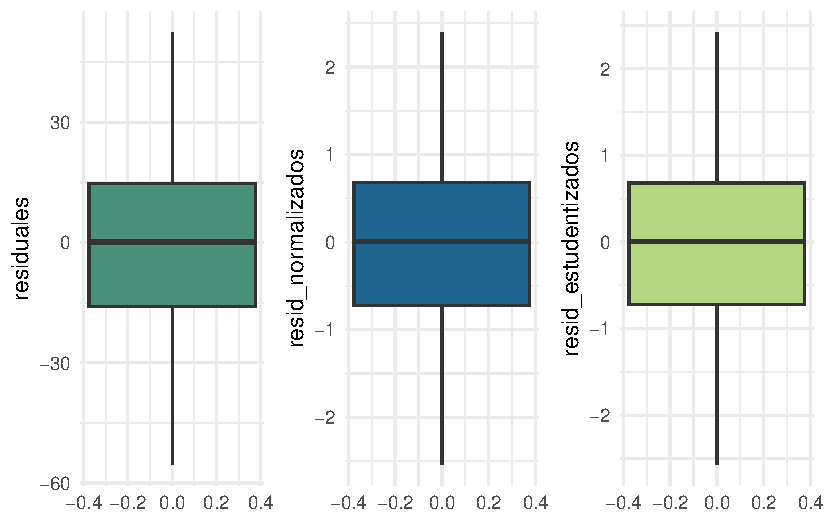
\includegraphics{index_files/figure-pdf/unnamed-chunk-36-1.pdf}
\end{center}

Observamos que existen residuales atípicos que se repiten en las tres
gráficas, aunque ninguno es mayor o menor a 3 desvíos en el boxplot de
los residuos estudentizados.

Si pretendiésemos conocer que valores tienen las variables de la
observación con residual mayor a 3 desvíos estándar, basta con hacer lo
siguiente:

\begin{Shaded}
\begin{Highlighting}[]
\CommentTok{\# detectamos observaciones mayor a 3 ds}
\FunctionTok{table}\NormalTok{(}\FunctionTok{rstudent}\NormalTok{(modelo) }\SpecialCharTok{\textgreater{}} \DecValTok{3}\NormalTok{)}
\end{Highlighting}
\end{Shaded}

\begin{verbatim}

FALSE 
  236 
\end{verbatim}

El hecho de que un valor sea atípico o con alto grado de \emph{leverage}
no implica que sea influyente en el conjunto del modelo. Sin embargo, si
un valor es influyente, suele ser o atípico o de alto \emph{leverage}.
Existen diferentes formas de evaluar la influencia de las observaciones:

\begin{itemize}
\item
  La \textbf{distancia de Cook} es una medida muy utilizada que combina,
  en un único valor, la magnitud del residual y el grado de leverage.
  Valores de Cook mayores a 1 suelen considerarse como influyentes.
\item
  Evaluar el cambio en los coeficientes de regresión tras excluir la
  observación: Se trata de un proceso iterativo en el que cada vez se
  excluye una observación distinta y se reajusta el modelo para
  comparar.
\end{itemize}

Esto lo podemos visualizar en el siguiente gráfico (\emph{Cook's
distance}) incluído en salida completa de \texttt{plot(modelo)}

\begin{Shaded}
\begin{Highlighting}[]
\FunctionTok{plot}\NormalTok{(modelo, }\AttributeTok{which =} \DecValTok{5}\NormalTok{)}
\end{Highlighting}
\end{Shaded}

\begin{center}
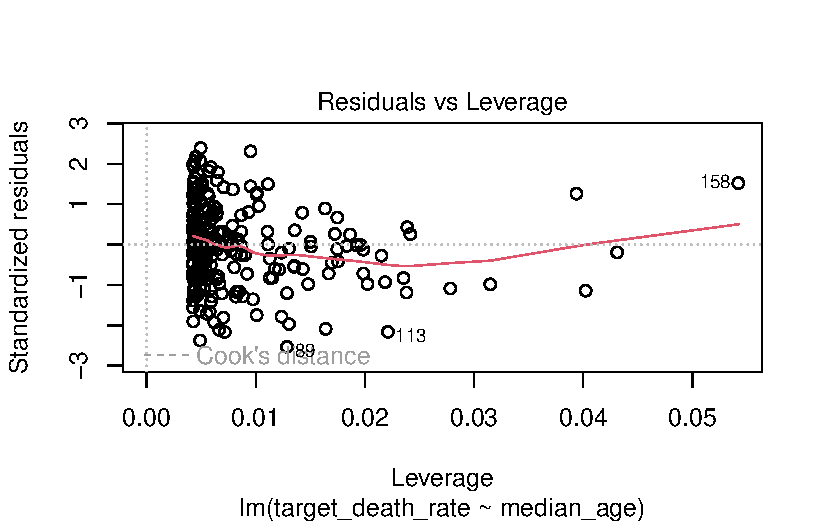
\includegraphics{index_files/figure-pdf/unnamed-chunk-38-1.pdf}
\end{center}

Al observar este gráfico, estaremos atentos a valores periféricos en la
esquina superior e inferior. Esos lugares, fuera de las líneas punteadas
rojas, son los lugares donde los puntos pueden ser influyentes contra
una línea de regresión.

Los casos que encontremos tienen altas puntuaciones de distancia de Cook
y por lo tanto influyen en los resultados de la regresión.

En caso de detectarse algún punto fuera de esos límites que establecen
las líneas discontinuas debe estudiarse este punto de forma aislada para
detectar, por ejemplo, si la elevada influencia de esa observación se
debe a un error.

En el ejemplo visualizado no encontramos evidentes valores influyentes.

El paquete \texttt{performance} incluye la función
\texttt{check\_outliers()} que permite detectar valores atípicos según
su distancia de Cook:

\begin{Shaded}
\begin{Highlighting}[]
\FunctionTok{check\_outliers}\NormalTok{(modelo) }
\end{Highlighting}
\end{Shaded}

\begin{verbatim}
OK: No outliers detected.
- Based on the following method and threshold: cook (0.7).
- For variable: (Whole model)
\end{verbatim}

En el caso de detectar algún valor de este tipo, sobre todo si es
severo, es importante investigarlo. Puede tratarse de un dato mal
registrado, o que fue mal transcripto a la base de datos. En tal caso
podremos eliminar la observación (o corregirla) y analizar los casos
restantes. Pero si el dato es correcto, quizás sea diferente de las
otras observaciones y encontrar las causas de este fenómeno puede llegar
a ser la parte más interesante del análisis. Por supuesto que todo esto
dependerá del contexto del problema que uno esta estudiando.

\subsubsection{Bondad de ajuste del
modelo}\label{bondad-de-ajuste-del-modelo}

Una vez que se ha ajustado un modelo es necesario verificar su
eficiencia, ya que aun siendo la línea que mejor se ajusta a las
observaciones de entre todas las posibles, el modelo puede ser malo. Las
medidas más utilizadas para medir la calidad del ajuste son: error
estándar de los residuales, el test \(F\) y el coeficiente de
determinación \(R^2\).

Estos valores se encuentran en la parte final de la salida del
\texttt{summary(modelo)}, donde leemos RSE - error estandar de los
residuos (\textbf{Residual standar error}), coeficiente de determinación
\(R^2\) (\textbf{Multiple R-squared}) y \(R^2\) ajustado
(\textbf{Adjusted R-squared}).

Podemos acceder al valor de \(R^2\) del modelo usando la función
\texttt{r2()} del paquete \texttt{performance}

\begin{Shaded}
\begin{Highlighting}[]
\FunctionTok{r2}\NormalTok{(modelo)}
\end{Highlighting}
\end{Shaded}

\begin{verbatim}
# R2 for Linear Regression
       R2: 0.018
  adj. R2: 0.014
\end{verbatim}

\(R^2\) oscila entre 0 y 1, de manera que, valores de \(R^2\) próximos a
1 indican un buen ajuste del modelo lineal a los datos. Por otro lado,
\(R^2\) ajustado es similar a \(R^2\), pero penaliza la introducción en
el modelo de variables independientes poco relevantes a la hora de
explicar la variable dependiente (se utiliza en modelos lineales
múltiples). Por tanto, \(R^2\) ajustado \textless{} = \(R^2\).

En nuestro ejemplo, \(R^2\) = 0.018 y \(R^2\) ajustado = 0.014; por lo
que podemos concluir que el modelo lineal simple no se ajusta demasiado
bien a nuestros datos.

Esto indica que aproximadamente el 1.4 \% de la variación en la tasa de
mortalidad por cáncer se puede explicar por el modelo que solo contiene
la mediana de edad como variable explicativa. Es bajo, por lo que las
predicciones de la ecuación de regresión son bastante poco confiables,
ya que también significa que hay otro 98.6 \% de la variación que aún no
se explica, por lo que quizás agregar otras variables independientes
podría mejorar el ajuste del modelo.

La última línea de la salida de \texttt{summary(modelo)} incluye un
estadístico de distribución continua \(F\) \emph{de Snedecor} (Test F) y
el \emph{valor} \(p\) correspondiente que se utilizan para resolver lo
que se conoce habitualmente como contraste ómnibus. Mediante este
contraste se comprueba si, de forma global, el modelo lineal es
apropiado para modelizar los datos.

En nuestro ejemplo, el \emph{p}-valor asociado a este contraste es
inferior a 0,05 por lo que, al 95\% de confianza podemos rechazar la
hipótesis nula y afirmar que, efectivamente, el modelo lineal es
adecuado para nuestro conjunto de datos.

Cuando el modelo de regresión tiene una única variable explicativa, el
contraste de la regresión es equivalente al contraste del parámetro
\(\beta_1\) (ciclistas).

Otra manera de verificar, en forma independiente, la significación del
modelo de regresión es por medio de la función \texttt{anova()} que
plantea el contraste de la regresión mediante el análisis de la
varianza.

\begin{Shaded}
\begin{Highlighting}[]
\FunctionTok{anova}\NormalTok{(modelo)}
\end{Highlighting}
\end{Shaded}

\begin{verbatim}
Analysis of Variance Table

Response: target_death_rate
            Df Sum Sq Mean Sq F value  Pr(>F)  
median_age   1   2084 2083.75  4.3211 0.03873 *
Residuals  234 112840  482.22                  
---
Signif. codes:  0 '***' 0.001 '**' 0.01 '*' 0.05 '.' 0.1 ' ' 1
\end{verbatim}

La tabla de analisis de varianza muestra el mismo resultado que el
bloque final de \texttt{summary(modelo)} con un valor F de 4.32 y un
\emph{p}-valor significativo.

\paragraph{Resumen del resultado del
ejemplo}\label{resumen-del-resultado-del-ejemplo}

Se llevó a cabo una regresión lineal simple para analizar la relación
entre la mediana de edad y la tasa de mortalidad por cáncer en 236
condados de Estados Unidos.

El diagrama de dispersión mostró una relación lineal negativa moderada
entre los dos, que se confirmó con un coeficiente de correlación de
Pearson de 0.25 . La regresión lineal simple mostró una relación
significativa entre las variables (t = -2.08 \emph{p} = 0.039).

El coeficiente de pendiente de la recta para la mediana de edad fue de
-0.57, por lo que la tasa de mortalidad por cáncer disminuye
aproximadamente 0,6 \% por cada unidad que sube la mediana de edad de
los pacientes.

El valor \(R^2\) mostró que el 1.4 \% de la variación en la tasa de
mortalidad por cáncer se puede explicar por el modelo que solo contiene
la mediana de edad.

La gráfica de dispersión de los valores pronosticados estandarizados
frente a los residuos estandarizados, mostró que los datos cumplían los
supuestos de homogeneidad de varianza y linealidad y que los residuos se
distribuían aproximadamente de forma normal.

Se cumplieron todos los presupuestos necesarios para validar la
regresión y no se encontraron valores atípicos influyentes.

\subsection*{Bibliografía}\label{bibliografuxeda}
\addcontentsline{toc}{subsection}{Bibliografía}

\phantomsection\label{refs}
\begin{CSLReferences}{1}{0}
\bibitem[\citeproctext]{ref-ballesterduxedez2003}
Ballester Díez, Ferrán, and José María Tenías Burillo. 2003.
\emph{Estudios Ecológicos}. Valencia : Escola Valenciana d{'}Estudis per
a la Salut, 2003.

\bibitem[\citeproctext]{ref-daniel2002}
Daniel, Wayne W. 2002. \emph{Bioestadística: Base Para El Análisis de
Las Ciencias de La Salud}. 4th ed. Limusa Wiley.

\bibitem[\citeproctext]{ref-escuelanacionaldesanidad}
Escuela Nacional de Sanidad (ENS). Instituto de Salud Carlos III.
Ministerio de Ciencias e Innovación. Madrid. 2009. \emph{Manual Docente
de La Escuela Nacional de Sanidad: Método Epidemiológico}.

\bibitem[\citeproctext]{ref-nortest}
Gross, Juergen, and Uwe Ligges. 2015. {``Nortest: Tests for
Normality.''} \url{https://CRAN.R-project.org/package=nortest}.

\bibitem[\citeproctext]{ref-hernuxe1ndez-uxe1vila2011}
Hernández-Ávila, Mauricio. 2011. \emph{Epidemiología: diseño y análisis
de estudios}. Buenos Aires: Editorial Médica Panamericana.

\bibitem[\citeproctext]{ref-performance}
Lüdecke, Daniel, Mattan S. Ben-Shachar, Indrajeet Patil, Philip
Waggoner, and Dominique Makowski. 2021.
{``{\textbraceleft}Performance{\textbraceright}: An
{\textbraceleft}r{\textbraceright} Package for Assessment, Comparison
and Testing of Statistical Models''} 6: 3139.
\url{https://doi.org/10.21105/joss.03139}.

\bibitem[\citeproctext]{ref-sheather2009}
Sheather, Simon. 2009. \emph{A Modern Approach to Regression with r}.
Springer Science \& Business Media.

\bibitem[\citeproctext]{ref-gtsummary}
Sjoberg, Daniel D., Karissa Whiting, Michael Curry, Jessica A. Lavery,
and Joseph Larmarange. 2021. {``Reproducible Summary Tables with the
Gtsummary Package''} 13: 570--80.
\url{https://doi.org/10.32614/RJ-2021-053}.

\bibitem[\citeproctext]{ref-triola2009}
Triola, Mario F. 2009. \emph{ESTADÍSTICA Decima Edicion}. Pearson
Educación de México, SA de CV.

\bibitem[\citeproctext]{ref-weisberg2005}
Weisberg, Sanford. 2005. \emph{Applied Linear Regression}. Vol. 528.
John Wiley \& Sons.

\bibitem[\citeproctext]{ref-tidyverse}
Wickham, Hadley, Mara Averick, Jennifer Bryan, Winston Chang, Lucy
D'Agostino McGowan, Romain François, Garrett Grolemund, et al. 2019.
{``Welcome to the {\textbraceleft}Tidyverse{\textbraceright}''} 4: 1686.
\url{https://doi.org/10.21105/joss.01686}.

\bibitem[\citeproctext]{ref-lmtest}
Zeileis, Achim, and Torsten Hothorn. 2002. {``Diagnostic Checking in
Regression Relationships''} 2.
\url{https://CRAN.R-project.org/doc/Rnews/}.

\end{CSLReferences}



\end{document}
